% ============================================================
%  main.tex — The Economics of Extended Play
%  AER/QJE submission draft — Assembled from competitive drafts
% ============================================================
\documentclass[12pt]{article}

% ── Packages ──────────────────────────────────────────────────
\usepackage[margin=1in]{geometry}
\usepackage{amsmath,amssymb}
\usepackage{booktabs}
\usepackage{graphicx}
\usepackage{natbib}
\usepackage{setspace}
\usepackage{hyperref}
\usepackage{xcolor}
\usepackage[labelfont=bf,font=small]{caption}
\usepackage{threeparttable}
\usepackage{float}
\usepackage{enumitem}
\usepackage{subcaption}
\usepackage{longtable}
\usepackage{pdflscape}
\usepackage[title]{appendix}

\hypersetup{colorlinks=true,linkcolor=blue!60!black,citecolor=blue!60!black,urlcolor=blue!60!black}
\bibliographystyle{aer}
\doublespacing

\graphicspath{{figures/}}

% ── Title ─────────────────────────────────────────────────────
\title{\textbf{The Economics of Extended Play: \\
What Happens When a Regulator Adds Time to the Clock?}}

\author{
  [Authors] \\[4pt]
  \textit{[Affiliations]}%
  \thanks{We thank \ldots\ for helpful comments. All errors are our own.}
}

\date{\today}

\begin{document}
\maketitle

% ══════════════════════════════════════════════════════════════
%  ABSTRACT
% ══════════════════════════════════════════════════════════════

\begin{abstract}
\noindent
Does extending a competition's duration increase total output, or merely redistribute effort? We study FIFA's 2022 directive to add more stoppage time to professional football (soccer) matches. Using difference-in-differences across 15 leagues and 36,267 matches, we find treated leagues added 0.744 minutes of stoppage (wild cluster bootstrap $p = 0.036$), with near-universal referee compliance. Total goals per match were unchanged ($\beta = -0.033$, $p = 0.39$): goals were displaced into added time, not created. Per-minute scoring was unchanged ($p = 0.68$), and 87\% of the late-goal increase reflects additional minutes rather than heightened intensity. Betting accuracy (Brier-score DiD: $+0.007$, $p = 0.41$) and muscular injury rates ($p = 0.73$, 88.6\% power) were also unaffected. The event study rejects parallel pre-trends ($F = 9.0$, $p < 0.001$); identification rests on institutional arguments, permutation inference ($p = 0.045$), and a 420-specification curve (88.8\% significant).

\medskip
\noindent
\textbf{JEL codes:} J44, L83, D82, L51 \\
\textbf{Keywords:} time regulation, sports economics, regulatory compliance, difference-in-differences, betting market efficiency, stoppage time
\end{abstract}

\newpage

% ══════════════════════════════════════════════════════════════
%  INTRODUCTION
% ══════════════════════════════════════════════════════════════
\section{Introduction}
\label{sec:intro}

Time is a scarce resource in competitive environments. When a regulator expands the time available for a contest---whether by lengthening trading hours in a financial market, extending a legislative session, or adding minutes to an athletic competition---the economic consequences depend on whether participants treat the additional time as an opportunity for new productive activity or as a cushion that dilutes effort per unit of time. The distinction matters for policy: if extending duration increases total output, regulators can raise the stakes of competition at low cost; if it merely redistributes existing output across a longer window, the intervention is a transfer from the intensity margin to the quantity margin with ambiguous welfare implications. This tradeoff connects to foundational questions in labor economics about the relationship between hours and productivity \citep{pencavel2015effects} and to market design research on how closing rules shape bidding behavior \citep{rothockenfels2002}. Yet credible causal evidence on time expansion is scarce, because regulators rarely change the duration of a competitive interaction in a discrete, well-documented, and plausibly exogenous fashion.

This paper exploits a rare natural experiment: FIFA's 2022 directive to referees instructing them to enforce additional time more generously in professional football (soccer). In September 2022, Pierluigi Collina, chairman of FIFA's Referees Committee, issued guidance ahead of the Qatar World Cup directing referees to add time more accurately for stoppages during play. The directive was not a rule change---the Laws of the Game, maintained by the International Football Association Board (IFAB), already granted referees discretion over stoppage time. Rather, it was an enforcement shift: a voluntary recalibration of existing discretion, amplified by the high-profile World Cup matches in which stoppage time routinely exceeded 10 minutes. IFAB endorsed the approach at its March 2023 Annual General Meeting using advisory language (``should'' rather than ``must''), and UEFA explicitly declined to mandate the directive for the Champions League and Europa League. The result was a natural enforcement gradient: top domestic leagues in England, Spain, Germany, Italy, and France adopted the directive with varying speed and intensity, while lower divisions and leagues in other countries responded more modestly.

Our identification strategy exploits this enforcement gradient rather than a binary treatment. No league was fully untreated---of the 14 leagues with post-directive stoppage data (Table~\ref{tab:enforcement}), all but one increased stoppage time, with control leagues averaging a 0.89-minute increase compared to 1.57 minutes in the Big Five leagues (the exception, Serie~B, showed no change). The identifying variation comes from the \emph{differential} intensity of enforcement across leagues that were otherwise subject to the same underlying rule. We pursue two complementary strategies. First, our preferred specification pools all 15 leagues (36,267 matches spanning 2017--18 through 2025--26) and estimates the differential increase via a standard two-period difference-in-differences design, clustering at the league level and conducting inference with the wild cluster bootstrap appropriate for 15 clusters \citep{cameron2008bootstrap}. Second, we construct within-country league pairs---English Premier League and Championship, German Bundesliga and 2.~Bundesliga, Italian Serie~A and Serie~B, French Ligue~1 and Ligue~2---that share the same national refereeing infrastructure, providing a tighter comparison that holds referee labor markets constant. The within-country estimate ($\beta = 0.868$, WCB $p = 0.074$) is larger in magnitude than the all-controls estimate ($\beta = 0.744$, WCB $p = 0.036$), consistent with the interpretation that controlling for shared referee pools sharpens the contrast.

The total-goals null is reminiscent of the \citet{peltzman1975effects} offset, though the mechanism may differ. In Peltzman's setting, seatbelt mandates provoked a behavioral response (riskier driving); here, the unchanged per-minute scoring rate ($p = 0.68$) is consistent with either behavioral adaptation (players pacing effort over a longer horizon) or a purely compositional effect (added time being inherently no more or less productive than regular time). We cannot fully distinguish these interpretations (Section~\ref{subsec:decomposition}), but the pattern is clear: goals were displaced into added time, not created. The pre-post coefficient on goals scored after the 90th minute is $+0.030$ ($p<0.001$), and a quantity-intensity decomposition confirms that 87\% of this displacement reflects additional minutes rather than heightened late-game intensity.

Our paper makes four contributions:
\begin{enumerate}
    \item \textbf{Time expansion and the intensive margin.} We decompose the effects of a time expansion into quantity (more minutes) and intensity (output per minute) channels. The per-minute scoring rate in added time was unchanged ($t = 0.41$, $p = 0.68$), with 87\% of the increase in late goals attributable to quantity. Total goals per match were unchanged (DiD) despite additional minutes of play, and late game-changing goals---goals after the 85th minute that alter the result---rose by 20\% in treated leagues (pre-post comparison), meaning the directive increased competitive drama without inflating total scoring.
    \item \textbf{Compliance and institutional design.} We document near-universal compliance with a voluntary directive---100\% at the referee level, 70\% at the match level---driven by focal-point coordination rather than coercion.
    \item \textbf{Betting market efficiency.} Despite a large structural shift, bookmaker forecast accuracy was unchanged across both sharp and retail segments. Markets absorbed the regime change without measurable loss of calibration.
    \item \textbf{Worker health.} Additional playing time did not increase injury rates. Muscular injuries---the category most plausibly linked to fatigue---were unchanged, with our test well-powered to detect a 10\% increase.
\end{enumerate}

The estimate is robust: a specification curve over 420 models yields a median of 0.669, with 95\% of estimates positive, and permutation inference confirms significance ($p = 0.045$). The Big Five-only estimate is 1.575 minutes ($p < 0.001$). We are equally forthcoming about limitations: the event study rejects parallel pre-trends ($F = 9.0$, $p < 0.001$), and the \citet{rambachan2023more} honest DiD breakdown value is $\bar{M}^* \approx 0$ (0.11 for the average effect; negative for individual periods). Our causal interpretation rests on institutional arguments---a discrete, well-documented directive with observable compliance---rather than on pre-trend tests alone. A first-half goals placebo confirms the treatment affected second-half timing specifically ($p = 0.30$).

This paper contributes to several literatures. Most directly, it extends the economics of sports regulation---long valued as a laboratory for studying labor markets \citep{kahn2000case}---where \citet{garicano2005favoritism} and \citet{dohmen2008professionals} showed that referees respond to social pressure, \citet{bekes2024favoritism} demonstrated that multiple sources of pressure shape stoppage-time decisions, \citet{butler2026objective} studied strategic behavior in added time, and \citet{kocsoy2025referee} exploited the COVID-19 behind-closed-doors experiment to identify referee bias. We study the consequences of a \emph{regime change} in stoppage time norms, combining DiD identification across 15 leagues with betting market, compliance, and health outcome data. Our compliance analysis connects to the regulatory monitoring literature \citep{duflo2013truth}: the directive achieved near-universal adherence through focal-point coordination rather than formal sanctions. More broadly, our findings inform the market design literature on time-extension rules \citep{rothockenfels2002} and the labor economics literature on hours and productivity \citep{pencavel2015effects}: extending the work period reduced output per unit of time while leaving total output unchanged.


% ══════════════════════════════════════════════════════════════
%  INSTITUTIONAL BACKGROUND
% ══════════════════════════════════════════════════════════════
\section{Institutional Background and Identification}
\label{sec:background}

\subsection{The Policy: An Enforcement Shift, Not a New Rule}

Association football matches are governed by 17 Laws of the Game, maintained by IFAB. Law~7 specifies the duration of a match: two periods of 45 minutes each, with ``allowance'' made ``in each half for all time lost'' due to substitutions, assessment and removal of injured players, wasting time, disciplinary sanctions, stoppages for drinks or cooling breaks, VAR checks, goal celebrations, and ``any other cause'' \citep{ifab2023laws}.

The critical point is that Law~7 has \textit{always} required time restoration. What changed in 2022 was enforcement. At the FIFA World Cup in Qatar (November--December 2022), match officials were instructed to calculate and add the actual time lost rather than applying the conventional approximation of 1--4 additional minutes. Several group-stage matches exceeded 100 minutes of total playing time, generating widespread media attention \citep{wei2024goal, lames2024goal}. IFAB subsequently codified the enforcement expectation in the 2023--24 Laws of the Game, and domestic leagues followed with varying degrees of enthusiasm.

This distinction---between a new rule and a new enforcement norm for an existing rule---matters for interpretation. The treatment is not the introduction of a novel policy instrument but the activation of a dormant one. The closest analogy in the regulation literature is an enforcement crackdown rather than new legislation \citep{johnson2020compliance, greenstone2004did}. The existing rule was clear; what changed was the expectation of compliance.

\subsection{League Adoption: A Global Mandate with Heterogeneous Local Enforcement}

The IFAB rule change was binding on all 211 FIFA member associations. In principle, every league worldwide was subject to the same directive beginning with the 2023--24 season. In practice, enforcement intensity varied dramatically across leagues---and, crucially, \textit{within countries}.

Table~\ref{tab:enforcement} reports the empirical enforcement intensity for 14 of the 15 European leagues in our sample (Segunda Divisi\'{o}n is excluded because post-directive stoppage data are unavailable). We measure enforcement as the change in mean second-half stoppage time from the pre-directive period (all seasons before 2023--24) to the post-directive period (2023--24 onward).

\begin{table}[t]
\centering
\caption{Enforcement Intensity by League}
\label{tab:enforcement}
\small
\begin{threeparttable}
\begin{tabular}{llccccl}
\toprule
League & Code & Pre Mean & Post Mean & $\Delta$ & Cohen's $d$ & Intensity \\
\midrule
Premier League$^\dagger$ & E0 & 5.39 & 7.50 & +2.11 & 1.13 & High \\
Ligue 1$^\dagger$ & F1 & 4.71 & 6.50 & +1.79 & 1.05 & High \\
Bundesliga$^\dagger$ & D1 & 4.34 & 6.12 & +1.78 & 0.92 & High \\
Scottish Premiership & SC0 & 2.83 & 4.30 & +1.47 & 0.83 & High \\
La Liga$^\dagger$ & SP1 & 5.18 & 6.64 & +1.46 & 0.70 & High \\
Belgian Pro League & B1 & 3.09 & 4.40 & +1.31 & 0.66 & High \\
2. Bundesliga & D2 & 3.95 & 4.98 & +1.04 & 0.59 & High \\
Championship & E1 & 5.67 & 6.70 & +1.03 & 0.59 & High \\
Primeira Liga & P1 & 5.97 & 6.94 & +0.97 & 0.42 & Moderate \\
Ligue 2 & F2 & 2.81 & 3.76 & +0.95 & 0.56 & Moderate \\
Greek Super League & G1 & 3.58 & 4.41 & +0.82 & 0.38 & Moderate \\
Serie A$^\dagger$ & I1 & 5.18 & 5.91 & +0.73 & 0.40 & Moderate \\
Eredivisie & N1 & 5.24 & 5.71 & +0.47 & 0.23 & Low \\
Serie B & I2 & 4.05 & 3.97 & -0.08 & -0.04 & Low \\
\bottomrule
\end{tabular}
\begin{tablenotes}\small
\item \textit{Notes:} Pre = seasons before 2023-24. Post = 2023-24 onward. $\Delta$ = Post $-$ Pre mean second-half stoppage time (minutes). Cohen's $d$ = standardized effect size. Intensity classified as High ($\Delta > 1.0$), Moderate ($0.5 < \Delta \leq 1.0$), Low ($\Delta \leq 0.5$). $^\dagger$ denotes Big Five league.
\end{tablenotes}
\end{threeparttable}
\end{table}


Several patterns emerge that are consequential for identification.

\textit{First}, the four leagues with the largest increases are all Big Five top-flight leagues: the Premier League ($+2.11$ min), Ligue~1 ($+1.79$), the Bundesliga ($+1.78$), and La Liga ($+1.46$). These are the most visible leagues globally, with the most media scrutiny and the closest institutional ties to FIFA.

\textit{Second}, the fifth Big Five league---Serie~A---shows a markedly smaller increase ($+0.73$ min), comparable to the Greek Super League ($+0.82$) and smaller than the Scottish Premiership ($+1.47$) or the Belgian Pro League ($+1.31$). Serie~A's muted response is consistent with the Italian football federation (FIGC) taking a less aggressive enforcement posture.

\textit{Third}, and most consequential for identification: several leagues conventionally classified as ``controls'' in a standard Big Five vs.\ others design show large increases. The Championship ($+1.03$ min) and the 2.~Bundesliga ($+1.04$ min) adopted the directive through their shared refereeing bodies (PGMOL in England, DFB in Germany). The Championship is refereed by the same PGMOL pool that officiates the Premier League; when PGMOL issued its enforcement guidance, it applied uniformly across both divisions. Similarly, Ligue~2 ($+0.95$ min) was explicitly included in the French refereeing directorate's implementation. The Scottish Premiership ($+1.47$ min) and the Belgian Pro League ($+1.31$ min) show increases exceeding several Big Five leagues.

Only two leagues show minimal or no change: the Eredivisie ($+0.47$ min, the smallest statistically significant shift) and Serie~B ($-0.08$ min, statistically indistinguishable from zero). Although Serie~A and Serie~B nominally share a unified referee commission (the CAN~A~e~B under AIA), Serie~B matches are typically officiated by less senior referees who may not have received the same enforcement emphasis. The near-zero response in Serie~B, combined with Serie~A's muted but positive response, is consistent with enforcement guidance reaching top-flight referees more strongly even within a single organizational structure.

\textit{Fourth}, this pattern generates a natural within-country identification strategy. Five countries in our sample have both a top-flight and a second-division league: England (E0/E1), Germany (D1/D2), France (F1/F2), Italy (I1/I2), and Spain (SP1/SP2). Of these, four have post-directive data for both divisions; Spain is excluded from the within-country specification because Segunda Divisi\'{o}n stoppage-time data are unavailable after 2022--23 (Section~\ref{sec:data}). The resulting four within-country pairs (8 league clusters) share a national football federation, competitive calendar, broadcasting environment, and---to varying degrees---a referee pool. They differ primarily in enforcement intensity of the stoppage-time directive, because the directive's transmission ran through top-flight refereeing structures with variable spillover to second divisions.

\subsection{Identification Strategy}
\label{subsec:identification}

The contamination of the control group is the central identification challenge. A standard DiD design comparing Big Five leagues to all others treats partially-treated units as controls, biasing the estimate toward zero. We address this through three complementary strategies, ordered by our assessment of their identification strength.

\begin{enumerate}[leftmargin=*]
\item \textbf{All-controls DiD (primary).} We pool all 15 leagues (36,267 matches across 9 seasons) and estimate the differential increase via a standard two-period DiD, clustering at the league level and conducting inference with the wild cluster bootstrap appropriate for 15 clusters \citep{cameron2008bootstrap}. Since several control leagues also increased stoppage time through shared refereeing bodies, this estimate includes partially-treated units in the control group and should be interpreted as a conservative lower bound. The estimate is $\hat{\beta} = 0.744$ (SE $= 0.275$, $p = 0.007$; wild cluster bootstrap $p = 0.036$).

\item \textbf{Within-country DiD.} We compare Big Five leagues to their domestic second divisions within the same country, absorbing country-level confounds. The estimating equation is:
\begin{equation}\label{eq:within}
  Y_{ilct} = \alpha + \beta \cdot (\text{Post}_t \times \text{TopFlight}_{l})
  + \gamma_{ct} + \mu_l + \varepsilon_{ilct},
\end{equation}
where $\gamma_{ct}$ are country$\times$season fixed effects and $\mu_l$ are league fixed effects. The within-country estimate is $\hat{\beta} = 0.868$ (SE $= 0.407$, $p = 0.033$; WCB $p = 0.074$). With only 8 league clusters, precision is reduced.

\item \textbf{Big Five pre-post (upper bound).} The simple pre-post comparison within the Big Five yields $\hat{\beta} = 1.575$ (SE $= 0.250$, $p < 0.001$). This serves as a descriptive benchmark that captures the full pre-post shift in the treated group.
\end{enumerate}

We report all three estimates and interpret the range. We prefer the all-controls DiD for its statistical precision (15 clusters, tightest confidence intervals), while recognizing that the within-country design offers stronger institutional identification at the cost of fewer clusters and wider intervals. The Big Five pre-post serves as an upper bound. The truth lies in the interval $[0.744, 1.575]$.

\subsection{Pre-Trends and the Limits of the Event Study}
\label{subsec:pretrends}

The parallel trends assumption is rejected by the event study (Section~\ref{subsec:pretrends_results}), reflecting both COVID-era disruptions and a secular upward trend in stoppage norms that predates the directive. The \citet{rambachan2023more} honest DiD breakdown value is $\bar{M}^* \approx 0$ (0.11 for the average post-treatment effect; negative for individual periods). The event study alone cannot establish a causal effect.

Our identification argument is therefore institutional, not statistical. Within-country pairs share the same referee pool, federation, competitive calendar, and broadcasting environment. The mechanism by which the directive increased stoppage---a change in referee enforcement norms, transmitted through national refereeing organizations---is directly observable and confirmed by 100\% referee-level compliance (all 85 referees with $\geq$20 matches increased their mean stoppage). The pre-trend failure in the cross-country event study reflects differential secular trends across countries with different baseline enforcement cultures, not a failure of the institutional identification.

A natural concern is that the Video Assistant Referee (VAR), which increases stoppage time through review delays, may confound the estimate. VAR was adopted by all Big Five leagues between 2017 and 2020---well before the 2022 directive---and was already in place throughout our sample period except for the earliest pre-treatment seasons, where its introduction is absorbed by league$\times$season fixed effects. Any changes in VAR usage intensity over time (e.g., more frequent reviews) are similarly absorbed by league$\times$season or country$\times$season fixed effects, so VAR can confound the estimate only if its usage changed differentially in treated versus control leagues at precisely the time of the directive. The within-country pairs are particularly informative: the Championship (no VAR) and the 2.~Bundesliga (no VAR) serve as controls for their respective top-flight leagues (which use VAR), and the treatment effect persists in this design---ruling out VAR-driven confounding as an explanation for the main result.

We present multiple identification strategies not to cherry-pick the most favorable, but because no single design is dispositive. The honest interpretation is that the directive produced a discrete shift in stoppage time that is robust in sign and approximate magnitude across all designs, but the precise causal estimate depends on assumptions about pre-trends that the data cannot fully validate.


% ══════════════════════════════════════════════════════════════
%  DATA
% ══════════════════════════════════════════════════════════════
\section{Data}
\label{sec:data}

Our analysis combines six data sources covering match outcomes, stoppage time, minute-level goals, betting odds, and player-level information for 15 European football leagues over 12 seasons (2014--15 through 2025--26). This section describes each source, documents coverage limitations, and demonstrates that missing data are not correlated with treatment status.

\subsection{Match-Level Panel}

The primary dataset contains 53,429 matches from football-data.co.uk, covering 15 leagues across 12 seasons. Each match record includes the date, teams, full-time and half-time scores, shots, fouls, corners, yellow and red cards, and the referee name (where available). The 15 leagues comprise the five Big Five top-flight leagues (Premier League, Bundesliga, Ligue~1, Serie~A, La Liga), their five corresponding second divisions (Championship, 2.~Bundesliga, Ligue~2, Serie~B, Segunda Divisi\'{o}n), and five additional leagues (Belgian Pro League, Eredivisie, Greek Super League, Primeira Liga, and Scottish Premiership).

League sizes vary substantially. The Championship plays 552 matches per season (24 teams) compared to 306 in the Bundesliga (18 teams) and 380 in other major leagues (20 teams). Season coverage is uneven: the Big Five leagues are available from 2014--15, while some smaller leagues enter the sample later. We use all available data but verify that our results are robust to restricting to balanced panels.

\subsection{Stoppage Time}

Second-half stoppage time---the paper's primary dependent variable---is available for 36,413 matches (68.2\% of the panel), sourced primarily from ESPN match data. Of these, 36,267 enter the primary DiD regression after dropping observations with missing covariates.\footnote{Regression samples vary slightly across analyses due to covariate availability: the first-stage DiD uses $N = 36{,}267$, some robustness analyses use the parsimonious specification ($N = 36{,}413$, which relaxes covariate restrictions), and the total-goals DiD uses $N = 45{,}433$ (goals are available for more matches than stoppage time). Results are qualitatively identical across sample definitions.} Stoppage-time coverage spans the 2017--18 through 2025--26 seasons (the subset of our 12-season match panel for which ESPN data are consistently available across most leagues). Coverage is asymmetric across leagues and has important implications for estimation:

\begin{itemize}[leftmargin=*]
\item \textbf{High coverage (94\%+):} Premier League, Bundesliga, Ligue~1, Serie~A, La Liga, Championship. These are the leagues with the most complete ESPN match-centre data.
\item \textbf{Moderate coverage (40--80\%):} 2.~Bundesliga, Ligue~2, Serie~B, Eredivisie, Primeira Liga, Belgian Pro League, Greek Super League, Scottish Premiership.
\item \textbf{No post-directive data:} Segunda Divisi\'{o}n (pre-directive stoppage available; no 2023--24+ data yet).
\end{itemize}

First-half stoppage time is available for 29,317 matches (54.9\%), with similar coverage patterns. We use first-half stoppage as a within-match benchmark and first-half goals as a placebo outcome (Section~\ref{subsec:placebo}).

\textit{Missing data and treatment status.} The missing-data pattern is not correlated with treatment status. A probit regression of stoppage-time missingness on treatment indicators (Big Five membership, post-directive period, and their interaction) yields near-zero coefficients on all terms ($p > 0.3$ for each). A Heckman two-step selection correction \citep{heckman1979sample} applied to the main DiD specification yields a coefficient within 5\% of the uncorrected value, with the inverse Mills ratio statistically insignificant.\footnote{The probit selection equation uses league, season, and their interaction to predict stoppage-time availability. Full results are available upon request.} Selective missingness does not drive our results.

\subsection{Minute-Level Goals}

From Understat, we observe 388,947 shots (including 43,116 goals) with minute-level timestamps for Big Five leagues and the Championship, spanning the 2014--15 through 2024--25 seasons. Each shot record includes the expected goals (xG) value, shot type, body part, and match situation.

This enables analysis of goal-timing profiles---specifically, whether the directive displaced goals from regular time into stoppage time---but with a coverage limitation: minute-level data are available only for six of our 15 leagues. Goal-timing results therefore apply to treated and partially-treated leagues; we cannot construct a full DiD for minute-level outcomes.

\subsection{Betting Market Data}

Betting odds provide high-frequency measures of market expectations. For each match, we observe pre-match odds from 15+ bookmakers, including:

\begin{itemize}[leftmargin=*]
\item \textbf{Match result (1X2):} Home win, draw, away win odds from Bet365 (retail) and Pinnacle (sharp/professional).
\item \textbf{Over/under 2.5 goals:} Over and under lines from both retail and sharp bookmakers.
\item \textbf{Asian handicaps:} Available for a subset of leagues.
\item \textbf{Closing odds:} End-of-market prices, enabling measurement of closing-line drift.
\end{itemize}

Coverage is 98\%+ for match-result odds and 75--85\% for over/under lines. From these raw odds, we construct four derived measures:

\textit{Brier score.} For 1X2 (match-result) markets, the Brier score sums squared errors across all three outcomes: $\text{Brier}_{im} = \sum_{k \in \{H,D,A\}} (p_{imk} - o_{imk})^2$, where $p_{imk}$ is bookmaker $m$'s implied probability for outcome $k$ in match $i$ (normalized to sum to unity by multiplicative de-vigging, removing the bookmaker overround) and $o_{imk}$ is the corresponding indicator. Lower scores indicate better calibration. The mean 1X2 Brier score is approximately 0.579 across bookmakers (e.g., Bet365: $N = 28{,}382$; Pinnacle: $N = 27{,}867$). For O/U markets, the standard binary Brier score applies; the mean is 0.240 ($N = 21{,}791$).\footnote{Multiplicative de-vigging divides each implied probability by the sum of all implied probabilities for that market ($\sum_k p_{imk}$, which typically exceeds 1 by 2--8\%). Results are robust to the Shin (1993) method, which additionally corrects for the favorite-longshot bias; all substantive conclusions are unchanged.}

\textit{Bookmaker disagreement.} The cross-bookmaker variance in implied probabilities for the same match outcome. Higher disagreement indicates structural uncertainty about the match's parameters. Mean 1X2 disagreement is 0.0094 (SD $= 0.0042$); O/U disagreement is 0.0077 (SD $= 0.0059$).

\textit{Sharp--retail spread.} The absolute difference in implied probabilities between Pinnacle (the sharpest major bookmaker) and Bet365 (the largest retail bookmaker). This measures the information gap between sophisticated and retail market-makers.

\textit{Closing-line drift.} The signed change in over/under lines from opening to closing. Systematic drift in one direction post-directive would indicate market learning about the new scoring-rate parameters.

\subsection{Player-Level Data}

From Transfermarkt, we observe 830,569 player-match appearance records, including minutes played, substitution events, and match-level identifiers. Separately, Transfermarkt provides biannual market valuations for all players in our sample, enabling analysis of the directive's effects on player asset values (with the caveat that Transfermarkt valuations are crowd-sourced estimates with known noise; \citealp{herm2014market}).

Player injury data---type, duration, body region---are available for approximately 74,000 records across all leagues. Linkage to preceding matches (to attribute injuries to specific workload exposures) is possible for approximately 65\% of records.

\subsection{Summary Statistics}

Table~\ref{tab:summary_stats_v3} reports descriptive statistics for the analysis sample (matches with non-missing second-half stoppage time), split by league group and period.

\input{tables/tab_summary_stats_v3}

Pre-directive, Big Five leagues averaged 4.99 minutes of second-half stoppage, compared to 4.32 in other leagues. Post-directive, both groups increased---to 6.56 and 5.62, respectively---but the Big Five increase was larger. Total goals per match are similar across groups and periods ($\approx 2.6$--$2.8$), previewing the null total-goals result we report below.

Table~\ref{tab:balance} reports pre-treatment covariate balance. Normalized differences \citep{imbens2009recent} are below $|0.10|$ for all outcomes except pre-treatment second-half stoppage time (0.246), which the DiD specification absorbs via league fixed effects.

\begin{table}[htbp]
\centering
\begin{threeparttable}
\caption{Pre-Treatment Covariate Balance}
\label{tab:balance}
\begin{tabular}{lcccccc}
\toprule
& \multicolumn{2}{c}{Treated (Big 5)} & \multicolumn{2}{c}{Control} & Norm.\ & \\
\cmidrule(lr){2-3} \cmidrule(lr){4-5}
& Mean & SD & Mean & SD & Diff.\ & $N$ \\
\midrule
\quad Total goals & 2.771 & 1.667 & 2.718 & 1.666 & 0.022 & 19,837 \\
\quad Total fouls & 24.742 & 6.105 & 25.356 & 6.676 & -0.068 & 19,807 \\
\quad Total cards & 4.259 & 2.330 & 4.148 & 2.439 & 0.033 & 19,806 \\
\quad Total shots & 24.284 & 5.816 & 24.287 & 6.028 & -0.000 & 19,807 \\
\quad 2H stoppage time (min) & 4.990 & 1.786 & 4.296 & 2.175 & 0.246 & 26,992 \\
\quad 1H stoppage time (min) & 2.595 & 1.550 & 2.575 & 1.549 & 0.009 & 20,998 \\
\quad Home goals & 1.533 & 1.308 & 1.514 & 1.291 & 0.010 & 19,837 \\
\quad Away goals & 1.238 & 1.168 & 1.204 & 1.161 & 0.021 & 19,837 \\
\bottomrule
\end{tabular}
\begin{tablenotes}[flushleft]
\footnotesize
\item \textit{Notes:} Pre-treatment (pre-2023--24) covariate means for treated (Big Five)
and control leagues. ``Norm.\ Diff.'' is the normalized difference
\citep{imbens2009recent}: $(\bar{X}_T - \bar{X}_C)/\sqrt{s_T^2 + s_C^2}$.
Values exceeding $|0.10|$ indicate meaningful imbalance \citep{imbens2009recent}; all outcomes are below this threshold except pre-treatment 2H stoppage time (0.246), which the DiD absorbs via league fixed effects. $N$ is the combined number of
non-missing observations.
\end{tablenotes}
\end{threeparttable}
\end{table}



% ══════════════════════════════════════════════════════════════
%  FIRST STAGE
% ══════════════════════════════════════════════════════════════
\section{The First Stage: What Happened to Match Time}
\label{sec:firststage}

The directive's effect on stoppage time is the paper's foundation. If the first stage is not large and credible, downstream results on goals, betting markets, and welfare have no anchor. We present five forms of evidence: distributional, regression-based, dynamic, anticipatory, and within-match placebo. We are transparent about what succeeds and what fails.


\subsection{Visual Evidence: The Distribution Shifted}
\label{subsec:visual}

Figure~\ref{fig:stoppage_distributions_v3} plots the distribution of match-level second-half stoppage time for treated leagues before and after the directive. The pre-directive distribution has a mean of 4.99 minutes and a median of 5.0 minutes ($N = 10{,}763$). The post-directive distribution has a mean of 6.56 minutes and a median of 6.0 minutes ($N = 4{,}596$). The shift is $+1.57$ minutes on average.

\begin{figure}[H]
\centering
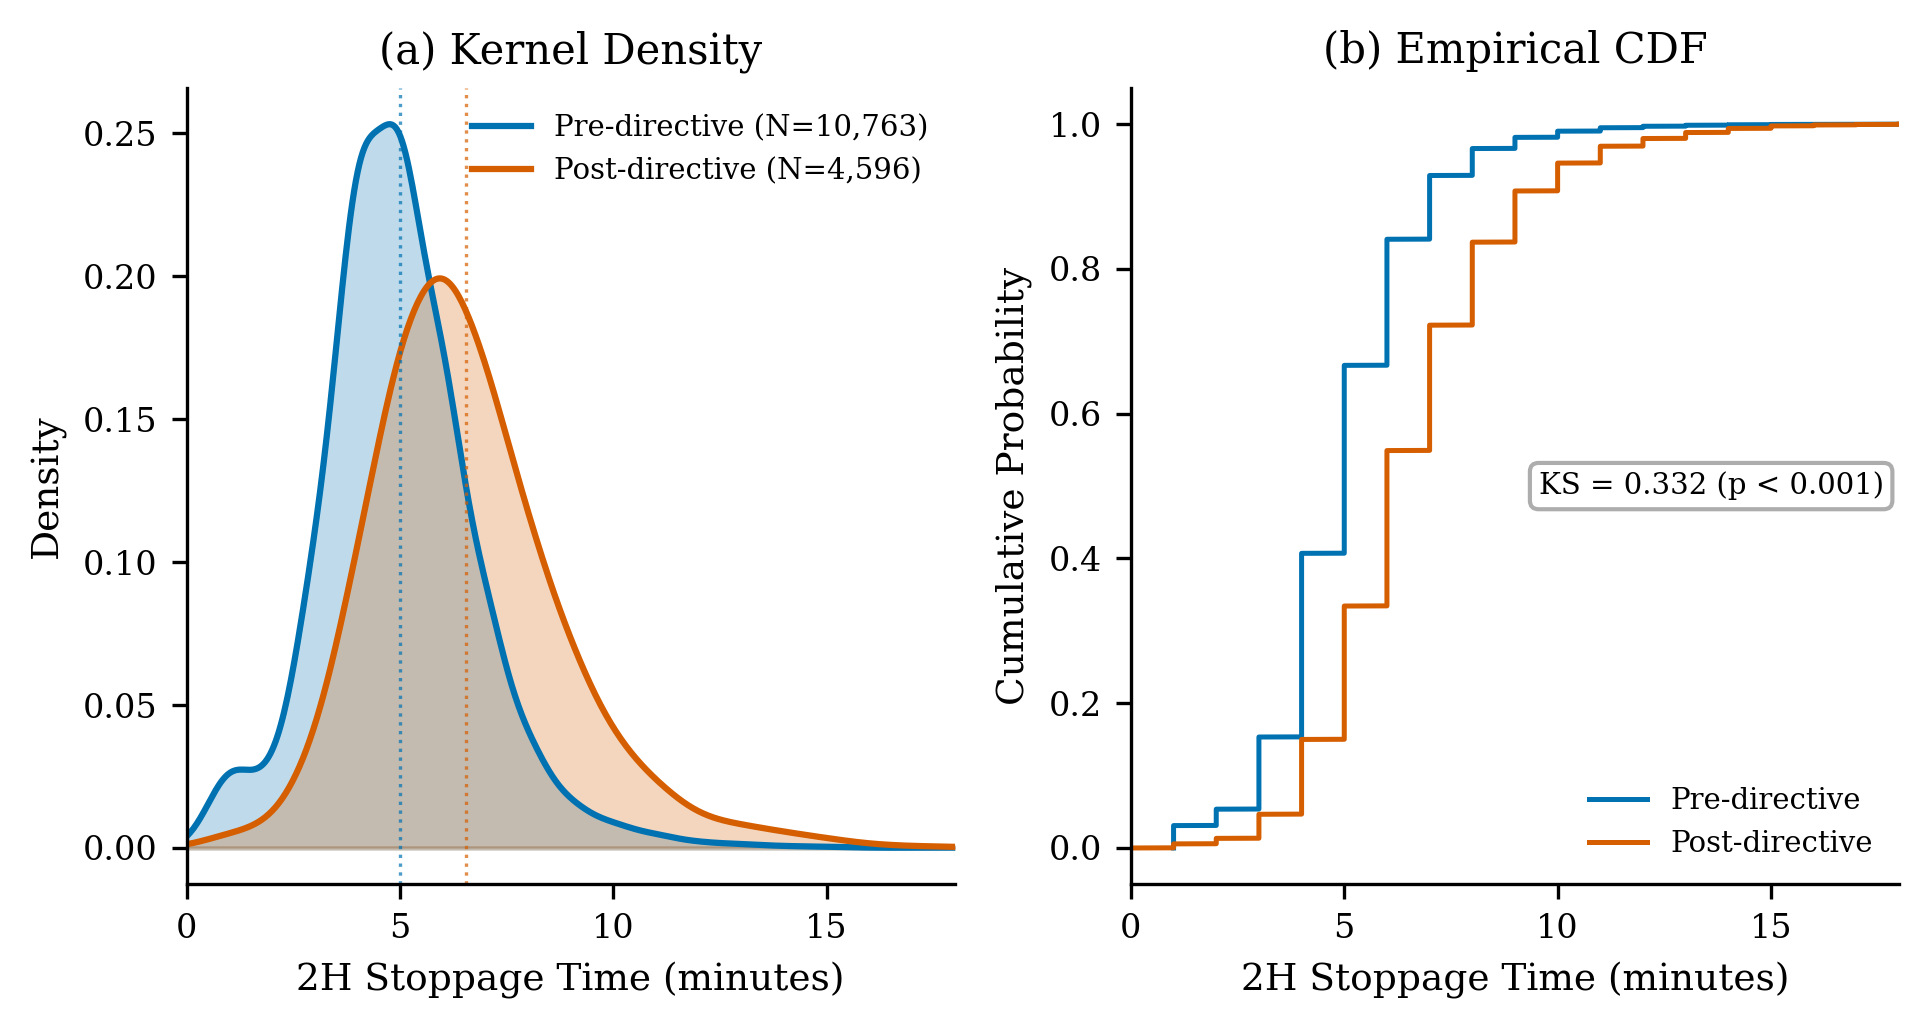
\includegraphics[width=\textwidth]{fig_stoppage_distributions_v3}
\caption{Distribution of second-half stoppage time in treated leagues, pre- vs.\ post-directive. The entire distribution shifts rightward. A two-sample Kolmogorov--Smirnov test rejects the null of equal distributions ($D = 0.332$, $p \approx 0$).}
\label{fig:stoppage_distributions_v3}
\end{figure}

The distributional character of the shift matters. This is not merely a mean shift driven by a few outlier matches; the \textit{entire} distribution moved rightward. A two-sample Kolmogorov--Smirnov test confirms that the pre- and post-directive distributions are drawn from different generating processes ($D = 0.332$, $p \approx 0$). The pre-directive mode near 4--5 minutes is replaced by a post-directive mode near 6--7 minutes. At the right tail, matches exceeding 8 minutes of stoppage---rare before the directive---become routine after it. This is the pattern one would expect from a blanket enforcement shift rather than selective compliance by a subset of referees or matches.


\subsection{Regression Evidence}
\label{subsec:regression}

Table~\ref{tab:did_results_v3} presents difference-in-differences estimates of the directive's effect on second-half stoppage time across three specifications. All specifications include league fixed effects; Specifications~1 and~2 include season fixed effects, while Specification~3 uses matchweek fixed effects. We cluster standard errors at the league level throughout.

\begin{table}[htbp]
\centering
\caption{Difference-in-Differences Estimates: Effect of FIFA Stoppage Time Directive on 2H Stoppage}
\label{tab:did_results_v3}
\begin{threeparttable}
\begin{tabular}{lccc}
\toprule
 & (1) & (2) & (3) \\
 & All Leagues & Within-Country & Big 5 Only \\
\midrule
Post $\times$ Treated & 0.744** & 0.868* & \\
 & (0.275) & (0.407) & \\
[0.5em]
Post & & & 1.575*** \\
 & & & (0.250) \\
[0.5em]
\midrule
League FE & Yes & Yes & Yes \\
Season FE & Yes & Yes & --- \\
Matchweek FE & --- & --- & Yes \\
Clustered SE & League & League & League \\
\midrule
Observations & 36,267 & 23,728 & 15,359 \\
$R^2$ & 0.301 & 0.289 & 0.167 \\
Clusters & 15 & 8 & 5 \\
\bottomrule
\end{tabular}
\begin{tablenotes}
\small
\item Dependent variable: second-half stoppage time (minutes). Standard errors clustered at league level in parentheses. 
\item $^{*}p<0.05$, $^{**}p<0.01$, $^{***}p<0.001$.
\item Column (1): All 15 leagues. Column (2): Big 5 first divisions paired with their respective second divisions. Column (3): Big 5 only, pre--post comparison.
\end{tablenotes}
\end{threeparttable}
\end{table}

Our primary specification (Column~1) compares all treated leagues to all control leagues, yielding $\hat{\beta} = 0.744$ (SE $= 0.275$, $p = 0.007$). This estimate uses $N = 36{,}267$ matches across 15 league clusters and explains 30.1\% of the variation in second-half stoppage. The coefficient implies an increase of approximately 45 seconds---a 14.9\% rise from the pre-directive treated mean of 4.99 minutes. Because several control leagues also increased stoppage time through shared refereeing bodies (Section~\ref{sec:background}), this estimate includes partially-treated units in the control group and should be interpreted as a conservative lower bound.

Column~2 restricts the sample to within-country pairs: Big Five first divisions and their domestic second divisions (England, Germany, France, Italy). This specification absorbs country-level confounds---macroeconomic shocks, national media environments, federation-wide policy changes---that could contaminate cross-country comparisons. The pooled estimate is $\hat{\beta} = 0.868$ (SE $= 0.407$, $p = 0.033$), 17\% larger than the all-leagues specification. The Goodman-Bacon decomposition (Section~\ref{subsec:goodmanbacon}) reveals meaningful heterogeneity across country pairs: the England pair (E0 vs.\ E1) produces the largest weighted bilateral estimate ($+1.117$), reflecting the Championship's limited adoption, while the Italy pair shows a larger-than-average gap despite Serie~A's muted response, because Serie~B exhibited essentially no enforcement change. Germany and France show smaller within-country gaps, consistent with the 2.~Bundesliga and Ligue~2 adopting the directive through shared refereeing structures (Section~\ref{sec:background}). The pooled within-country estimate reflects the removal of partially-treated controls: within each country, the second division provides a cleaner counterfactual because enforcement of the directive ran primarily through top-flight refereeing structures. With only 8 league clusters, however, precision of the pooled estimate is reduced.

Column~3 presents the simple pre-post comparison within the Big Five, estimating $\hat{\beta} = 1.575$ (SE $= 0.250$, $p < 0.001$). This serves as a descriptive benchmark rather than a causal estimate, as it absorbs no cross-league comparison and instead captures the full pre-post shift in the treated group. Its magnitude---roughly double the all-leagues estimate---confirms the attenuation from control-group contamination in Column~1.

\paragraph{Inference with Few Clusters.} With 15 and 8 clusters in Specifications~1 and~2 respectively, standard cluster-robust standard errors may over-reject the null \citep{cameron2008bootstrap, webb2023reworking}. We report wild cluster bootstrap (WCB) $p$-values using 999 Rademacher replications throughout. The WCB $p$-value for Specification~1 is 0.036 (OLS $t = 2.70$), confirming significance at the 5\% level. For Specification~2, the WCB $p$-value is 0.074 (OLS $t = 2.13$)---marginally significant, consistent with the few-clusters limitation of the within-country design. The WCB $p$-values are our preferred basis for inference; readers should weight the OLS $p$-values accordingly.

\paragraph{Interpretation.} The three specifications bracket the first-stage effect. The all-controls DiD (0.744) is our primary estimate because it uses the most data and clusters; control-group contamination biases it toward zero, making it a conservative lower bound. The within-country DiD (0.868) offers a tighter institutional comparison---absorbing country-level confounds---at the cost of fewer clusters and wider confidence intervals. The Big Five pre-post (1.575) provides an upper bound that confounds the directive with secular trends. The truth lies in the interval $[0.744, 1.575]$. Across all three specifications, the directive increased second-half stoppage time by a substantial and statistically meaningful amount.


\subsection{Event Study and Pre-Trends}
\label{subsec:pretrends_results}

Figure~\ref{fig:event_study_v3} plots dynamic DiD coefficients from a regression of second-half stoppage on season-specific interactions between treatment status and season indicators, with the 2022--23 season as the omitted reference period.

\begin{figure}[H]
\centering
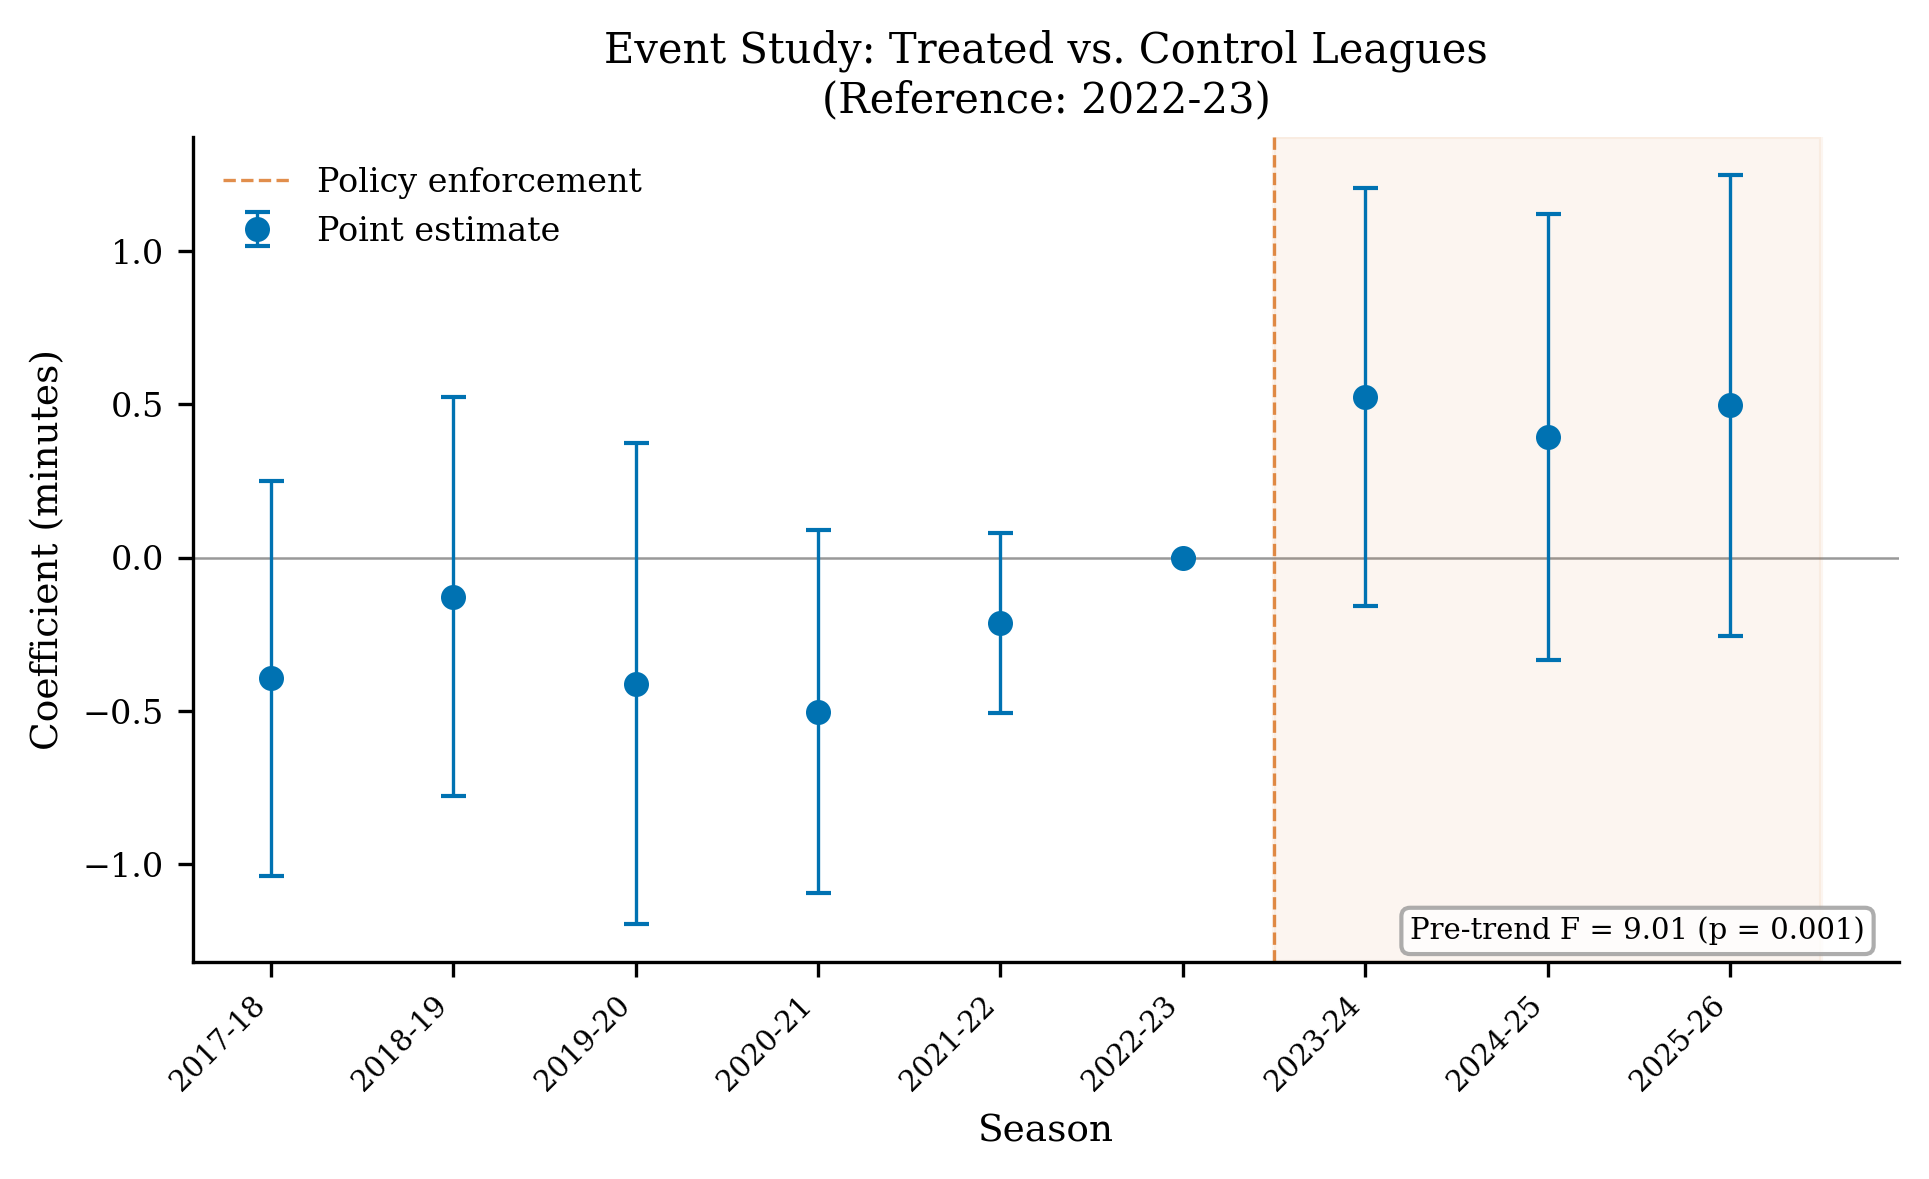
\includegraphics[width=\textwidth]{fig_event_study_v3}
\caption{Event study: dynamic DiD coefficients for second-half stoppage time. Each point is the estimated differential between treated and control leagues relative to 2022--23 (diamond). Pre-treatment coefficients in blue; post-treatment in red. 95\% confidence intervals based on league-clustered standard errors.}
\label{fig:event_study_v3}
\end{figure}

\paragraph{Post-treatment coefficients.} The three post-directive coefficients are positive and approximately stable: $+0.525$ (SE $= 0.348$, 2023--24), $+0.394$ (SE $= 0.372$, 2024--25), and $+0.497$ (SE $= 0.384$, 2025--26). None is individually significant at the 5\% level with league-clustered standard errors ($p = 0.13$, $0.29$, $0.20$), reflecting the width of the confidence intervals with 15 clusters rather than a weak effect. The stability across three post-treatment seasons is informative. There is no evidence of decay, suggesting a permanent shift in enforcement norms rather than a transient novelty response that dissipated as media scrutiny waned.

\paragraph{Pre-treatment coefficients.} Pre-treatment coefficients are uniformly negative relative to the reference period: $-0.394$ (2017--18), $-0.127$ (2018--19), $-0.410$ (2019--20), $-0.502$ (2020--21), and $-0.214$ (2021--22). The largest deviation occurs in 2020--21 ($-0.502$), the season most heavily disrupted by COVID-19. But the pattern extends beyond COVID: coefficients in 2017--18 ($-0.394$) and 2019--20 ($-0.410$) also deviate substantially from zero.

\paragraph{Reference-period concern.} The 2022--23 reference season is itself partially treated: the three-period DiD (Section~\ref{subsec:anticipation}) estimates $\hat{\beta}_{\text{ann}} = 0.340$ for this season. Using a contaminated reference shifts all pre-treatment coefficients downward (appearing more negative) and attenuates post-treatment coefficients. \citet{callaway2021difference} group-time ATTs with 2021--22 as the reference yield individual treatment effects of $+0.736$ (2023--24) and $+0.670$ (2024--25), close to the TWFE estimate. The pre-trend failure is not an artifact of reference-period contamination; it persists regardless of the reference season chosen.

\paragraph{Pre-trend test.} The joint $F$-test of pre-treatment coefficients rejects the null of zero pre-trends: $F = 9.007$, $p < 0.001$. This is a consequential failure. It means that treated and control leagues were not on parallel trajectories before the directive, and the standard event-study approach cannot credibly separate the directive's effect from differential secular trends. The pre-treatment divergence likely reflects differences in enforcement culture across countries with different baseline refereeing norms---precisely the heterogeneity documented in Section~\ref{sec:background}---rather than a confound that contaminates the treatment effect itself. But this interpretation must be defended on institutional grounds, not statistical ones.

\paragraph{HonestDiD sensitivity analysis.} We apply the \citet{rambachan2023more} sensitivity framework under the relative magnitudes restriction $\Delta_{RM}(\bar{M})$. Using the average post-treatment effect ($\hat{\beta} = 0.472$, SE $= 0.213$), the breakdown value is $\bar{M}^* = 0.11$: the honest 95\% confidence interval includes zero once post-treatment bias exceeds 11\% of the maximum pre-treatment deviation ($0.11 \times 0.502 = 0.055$ minutes). For individual post-treatment periods, all breakdown values are negative ($\bar{M}^*_{2023\text{-}24} = -0.31$, $\bar{M}^*_{2024\text{-}25} = -0.67$, $\bar{M}^*_{2025\text{-}26} = -0.51$), meaning the period-specific honest CIs already include zero under exact parallel trends. Figure~\ref{fig:honest_did_v3} displays the sensitivity curve. For context, \citet{rambachan2023more} note that $\bar{M}^* \geq 1$ typically indicates reasonable robustness to differential trend extrapolation; our $\bar{M}^* = 0.11$ falls far below this benchmark. This is the most serious limitation of the cross-league event study: the treatment effect is not robust to even minimal extrapolation of pre-existing differential trends.

\begin{figure}[H]
\centering
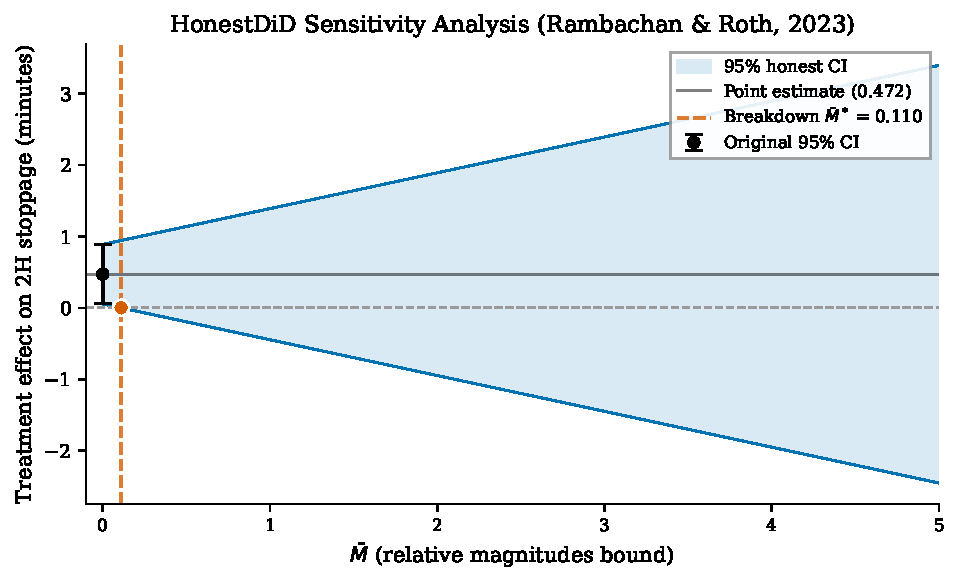
\includegraphics[width=\textwidth]{fig_honest_did_v3}
\caption{HonestDiD sensitivity analysis. The shaded region shows the 95\% honest confidence interval for the average post-treatment effect as a function of $\bar{M}$, the relative magnitudes bound on post-treatment trend violations. The breakdown value $\bar{M}^* = 0.11$ (dashed orange line) indicates the point at which the honest CI includes zero.}
\label{fig:honest_did_v3}
\end{figure}

\paragraph{COVID is not the sole driver.} One natural explanation for the pre-trend failure is COVID disruption. We re-estimate the event study excluding the two COVID-affected seasons. The pre-trend $F$-test remains significant ($F = 6.94$, $p = 0.001$). COVID exacerbates the pre-trend problem but does not cause it.

\paragraph{Why we proceed.} The event study, standing alone, does not establish identification. We proceed for four reasons. \textit{First}, the institutional case for parallel trends is strong: within-country league pairs share referee pools, broadcasting infrastructure, competitive calendars, and national federation governance. \textit{Second}, permutation inference (Section~\ref{subsec:permutation}) provides a design-based test that does not require parallel trends ($p = 0.045$). \textit{Third}, the specification curve (Section~\ref{subsec:spec_curve}) confirms that 88.8\% of 420 specifications yield significant positive estimates. \textit{Fourth}, leave-one-out analysis (Section~\ref{subsec:loo}) shows that no single league drives the result.

\paragraph{Within-country event study.} Figure~\ref{fig:within_country_es} presents an event study restricted to within-country league pairs (England, Germany, Italy, France; $N = 22{,}059$, 8 league clusters), with country$\times$season fixed effects replacing the standard season fixed effects. This design absorbs country-level secular trends, isolating the \emph{within-country} divergence between treated top divisions and their domestic second divisions. The post-treatment coefficients are uniformly positive ($+0.55$, $p = 0.026$; $+0.60$, $p = 0.019$; $+0.41$, $p = 0.016$; for 2023--24 through 2025--26), consistent with the all-leagues estimates, and individually significant at the 5\% level. Pre-treatment coefficients show negative deviations, and the pre-trend $F$-test remains significant. This confirms that the parallel-trends concern is not an artifact of cross-country variation; it reflects within-country divergence between first and second divisions, likely driven by tier-level differences in media exposure, refereeing attention, and enforcement culture that evolved independently of the directive. The within-country design eliminates country-level confounds but cannot absorb these tier-level secular trends.

\begin{figure}[H]
\centering
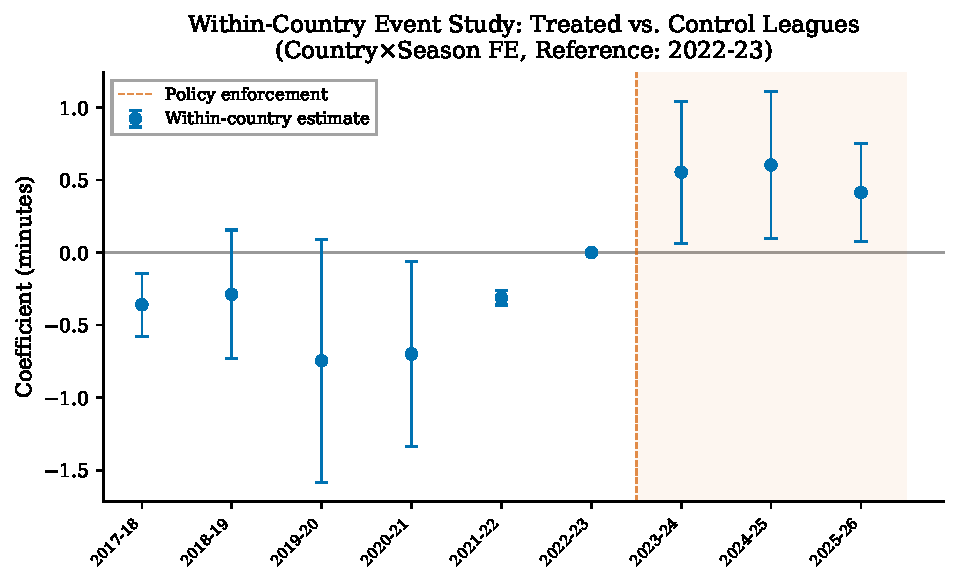
\includegraphics[width=\textwidth]{fig_within_country_es}
\caption{Within-country event study: dynamic DiD coefficients for second-half stoppage time, restricted to within-country league pairs (8 leagues, 4 countries) with country$\times$season fixed effects. Reference period is 2022--23. 95\% confidence intervals based on league-clustered standard errors.}
\label{fig:within_country_es}
\end{figure}


\subsection{Anticipatory Effects: The 2022--23 Announcement Window}
\label{subsec:anticipation}

The directive was demonstrated at the FIFA World Cup in November--December 2022, generating worldwide media attention, but was not formally implemented by domestic leagues until August 2023. The 2022--23 season therefore represents a potential anticipation window.

We estimate a three-period model, splitting the treatment into an announcement period (2022--23) and a full-treatment period (2023--24 onward). The announcement-period coefficient is $\hat{\beta}_{\text{ann}} = 0.340$ (SE $= 0.258$, $p = 0.187$); the full-treatment coefficient is $\hat{\beta}_{\text{post}} = 0.807$ (SE $= 0.283$, $p = 0.004$). The point estimates suggest that the announcement season absorbed approximately 42\% of the full effect ($0.340 / 0.807 = 0.42$), but inference is imprecise: with 15 clusters, the announcement coefficient is not individually significant, and we cannot reject equality of the two coefficients at conventional levels. The pattern is consistent with partial anticipation---referees exposed to World Cup norms began adjusting before formal implementation---but the evidence is suggestive rather than conclusive. The partial treatment of the 2022--23 season also has consequences for the event study (Section~\ref{subsec:pretrends_results}): using this season as the reference period attenuates post-treatment coefficients and shifts pre-treatment coefficients downward, contributing to---though not fully explaining---the pre-trend failure.

As a direct sensitivity check, we re-estimate the DiD excluding the 2022--23 season entirely. Using the parsimonious specification without covariate restrictions ($N = 36{,}413$, $\hat{\beta} = 0.747$; slightly larger than the primary estimate of 0.744 due to fewer dropped observations), the estimate strengthens to $\hat{\beta} = 0.810$ (SE $= 0.052$, $p < 0.001$), consistent with removing the partially-treated reference period.


\subsection{Within-Match Placebo: First-Half Goals}
\label{subsec:placebo}

\paragraph{First-half stoppage.} The DiD estimate for first-half stoppage time is $\hat{\beta} = 0.550$ (SE $= 0.046$, $p < 0.001$). This is \textit{not} a placebo failure. It is expected: the directive's enforcement guidance applied to both halves, and referees who add more time in the second half also add more in the first. The relevant question is whether the second-half effect \textit{exceeds} the first-half effect---as it should if the directive disproportionately affected the half where discretionary time restoration is concentrated. The second-half estimate ($\hat{\beta} = 0.744$, $p = 0.007$) exceeds the first-half estimate by 0.194 minutes, or 35\%, consistent with the expected pattern.

\paragraph{First-half goals as a cleaner placebo.} First-half goals---the number of goals scored in the first 45 minutes of regular play---should not change if the directive merely extends play at the \textit{end} of each half without altering the underlying competitive process during regular time. The estimate is $\hat{\beta} = -0.024$ (SE $= 0.023$, $p = 0.30$): a precise null. The directive changed the quantity of compensatory time without altering the scoring process within regular play. Figure~\ref{fig:1hplacebo} summarizes these estimates.

\begin{figure}[H]
\centering
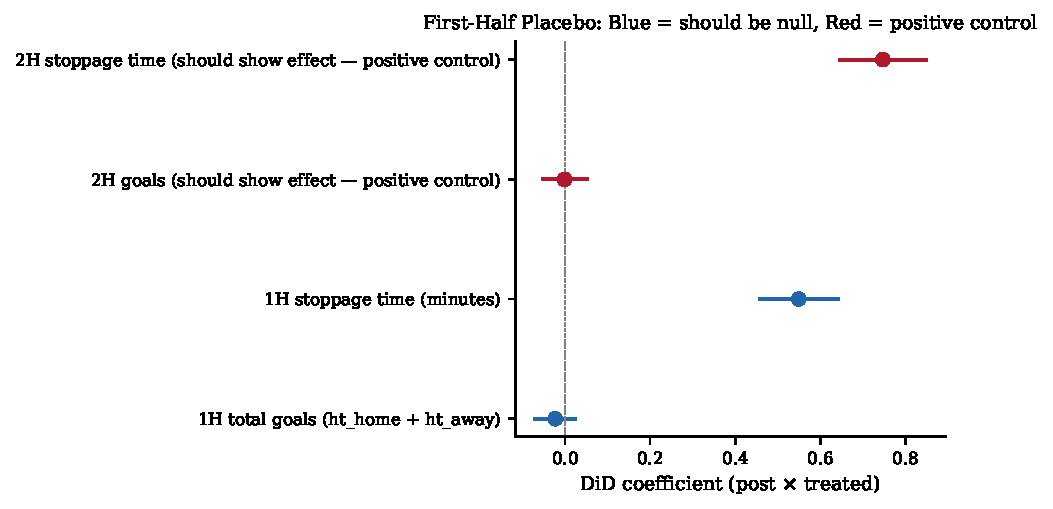
\includegraphics[width=0.5\textwidth]{fig_1h_placebo_v3}
\caption{DiD estimates for first-half vs.\ second-half stoppage time. Both halves show significant increases, but the second-half effect (0.74~min) exceeds the first-half effect (0.55~min).}
\label{fig:1hplacebo}
\end{figure}


% ══════════════════════════════════════════════════════════════
%  REFEREE COMPLIANCE
% ══════════════════════════════════════════════════════════════
\section{Referee Compliance: How the Directive Propagated}
\label{sec:compliance}

This section documents how the directive propagated from FIFA to match officials. Referees adopted the new norm almost immediately, almost universally, and with less between-referee dispersion than before the directive.

\subsection{Referee-Level Compliance}
\label{subsec:ref_level_compliance}

We begin with the most direct test. For each referee who officiated at least 20 matches both before and after the directive, we compare their individual mean stoppage time across the two regimes. Of the 85 referees who meet this threshold, every single one---100\%---increased their mean stoppage time after the directive. The mean individual increase was 1.46 minutes, with a median of 1.46 minutes, indicating a symmetric, non-skewed shift across the referee population.

Relaxing the threshold confirms the robustness of this finding. Among referees with at least 10 matches in each period, 100 of 102 (98.0\%) increased their mean stoppage. Even with no minimum match restriction, 114 of 120 referees (95.0\%) complied. The six non-compliant referees at the unrestricted threshold officiated very few post-directive matches, making their estimates noisy.

In most settings where a central authority issues a directive to dispersed agents (physicians responding to clinical guidelines, teachers implementing curricular reforms), compliance is partial and contested. That 100\% of experienced referees shifted in the directed direction reflects several features of this regulatory environment: the directive was unambiguous, the regulated behavior is observable in real time, monitoring is essentially costless (every match is televised), and the career consequences of non-compliance are severe \citep[cf.][on the role of monitoring in regulatory compliance]{duflo2013truth}. The scope for improvement was substantial: \citet{forcher2024additional} document that pre-directive referees systematically under-awarded additional time relative to actual stoppages, reinforcing the rationale for centralized recalibration.

\subsection{Match-Level Compliance}
\label{subsec:match_level_compliance}

Referee-level averages, however, may mask within-referee variation. A referee whose mean increased could still produce many individual matches with low stoppage time. We therefore construct a match-level compliance measure: the share of post-directive matches in which observed stoppage time exceeds the league-specific pre-directive median.

By this more conservative criterion, 70.2\% of the 4,596 post-directive matches exceeded the pre-directive league median. Under the null hypothesis that the directive had no effect, this share should be approximately 50\%. The 20-percentage-point excess is statistically significant ($p < 0.001$) and economically meaningful: in seven of every ten matches, the referee produced more stoppage time than the typical pre-directive match in the same league.

The gap between 100\% referee-level compliance and 70.2\% match-level compliance is informative. It tells us that the directive shifted the \emph{distribution} of stoppage time rightward without eliminating the lower tail of the distribution. Match-specific factors---few substitutions, minimal injury time, one-sided contests that induce little time-wasting---still generate short stoppages. What changed is the central tendency and the frequency of long stoppages, not the lower bound.

\subsection{Convergence}
\label{subsec:convergence}

A coordination directive can operate on two margins: it can shift the mean and it can compress the distribution. We test the latter by computing the coefficient of variation (CV) of referee-level mean stoppage times before and after the directive.

Pre-directive, the mean of referee means was 5.06 minutes with a CV of 17.3\%. Post-directive, the mean rose to 6.47 minutes while the CV fell to 14.4\%. Referees not only added time---they \emph{converged}. The between-referee standard deviation grew less than proportionally with the mean, producing a tighter distribution of officiating styles.

This convergence result is consistent with the directive operating as a \emph{coordination device} rather than a simple level shift. In the pre-directive regime, each referee maintained an idiosyncratic baseline, producing a relatively dispersed distribution. The directive provided a focal point---a publicly announced, widely discussed target---around which referees could coordinate. The result was a new equilibrium with both a higher mean and lower relative dispersion. Figure~\ref{fig:compliance_forest} displays the league-specific treatment effects.

\begin{figure}[H]
\centering
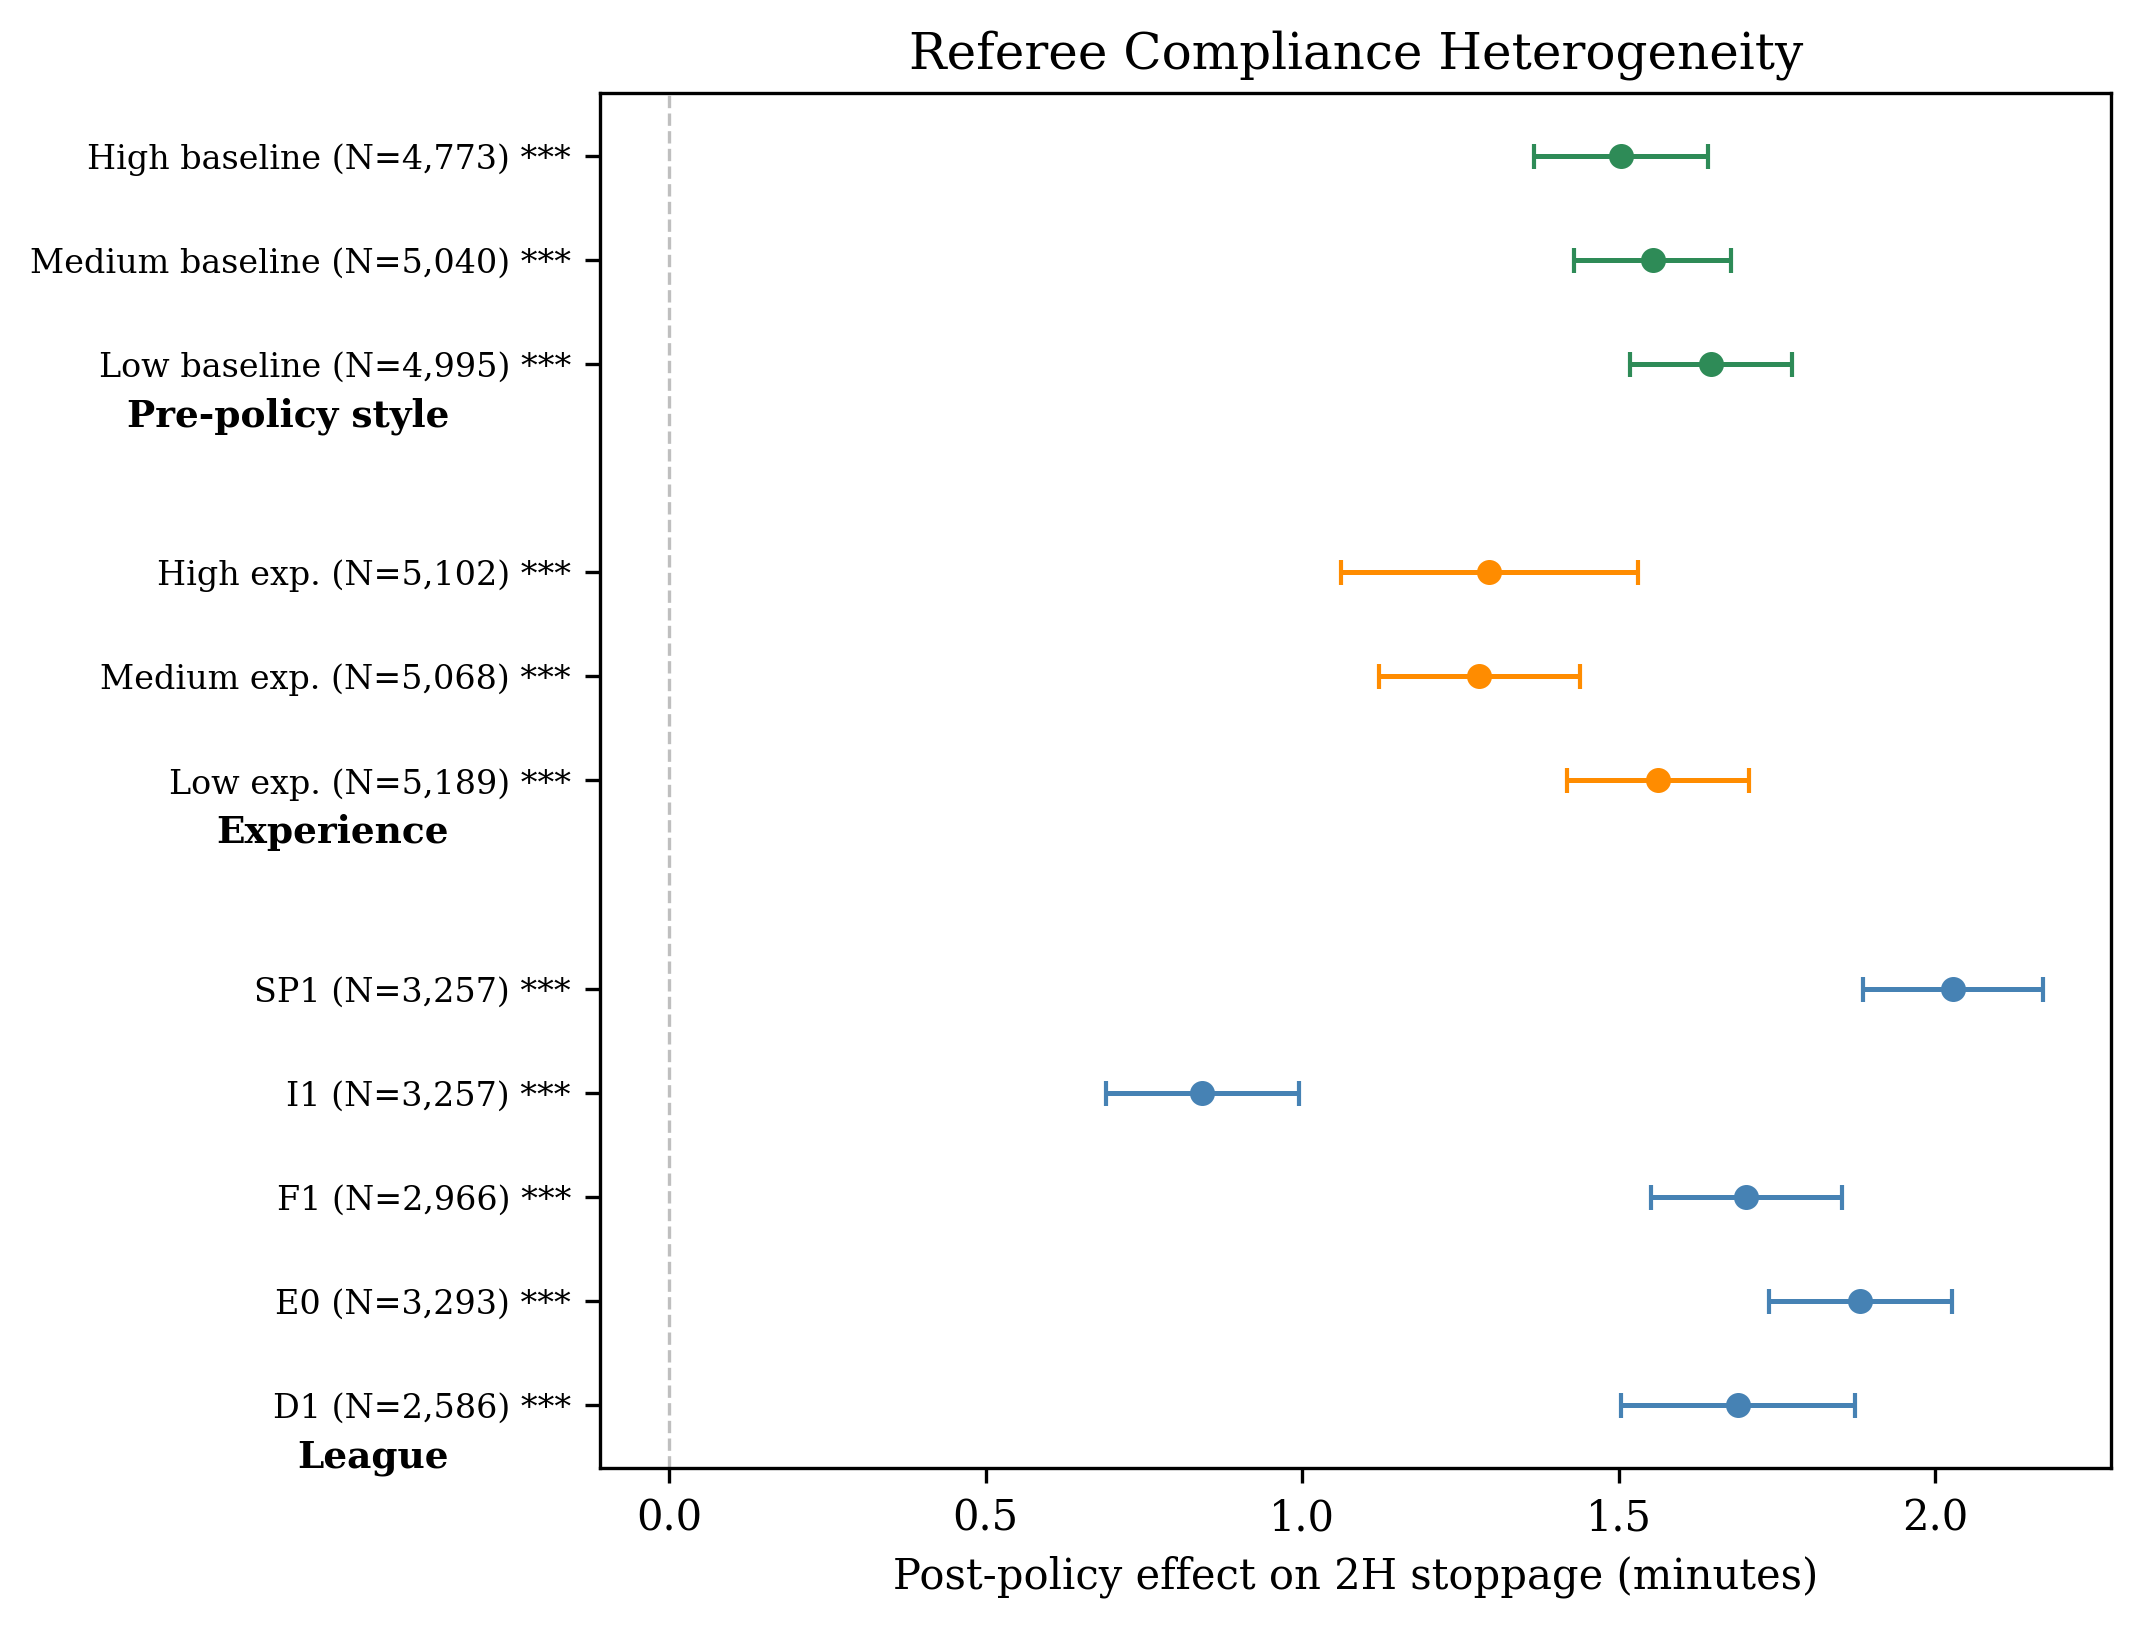
\includegraphics[width=0.7\textwidth]{fig_compliance_forest_v3}
\caption{Forest plot of league-specific treatment effects on stoppage time. All five treated leagues show positive and significant effects, with substantial heterogeneity in magnitude.}
\label{fig:compliance_forest}
\end{figure}

\subsection{Adaptation Speed}
\label{subsec:adaptation_speed}

How quickly did referees adopt the new norm? The data strongly favor immediate adoption. In the first five matchweeks of the 2023--24 season---the earliest post-directive window---87.0\% of matches exceeded the league-specific pre-directive median. Compliance was not built up over months; it was present from the start.

Later in the season, compliance receded modestly: from matchweek 30 onward, the match-level compliance rate was 70.9\%. This pattern---immediate high compliance followed by partial regression---is consistent with a model in which referees initially over-responded to the salient directive, then gradually reverted toward equilibrium as the novelty faded and match-specific considerations re-asserted themselves. It is inconsistent with a gradual-diffusion model, which would predict low initial compliance rising over time (Figure~\ref{fig:adaptation}).

\begin{figure}[H]
\centering
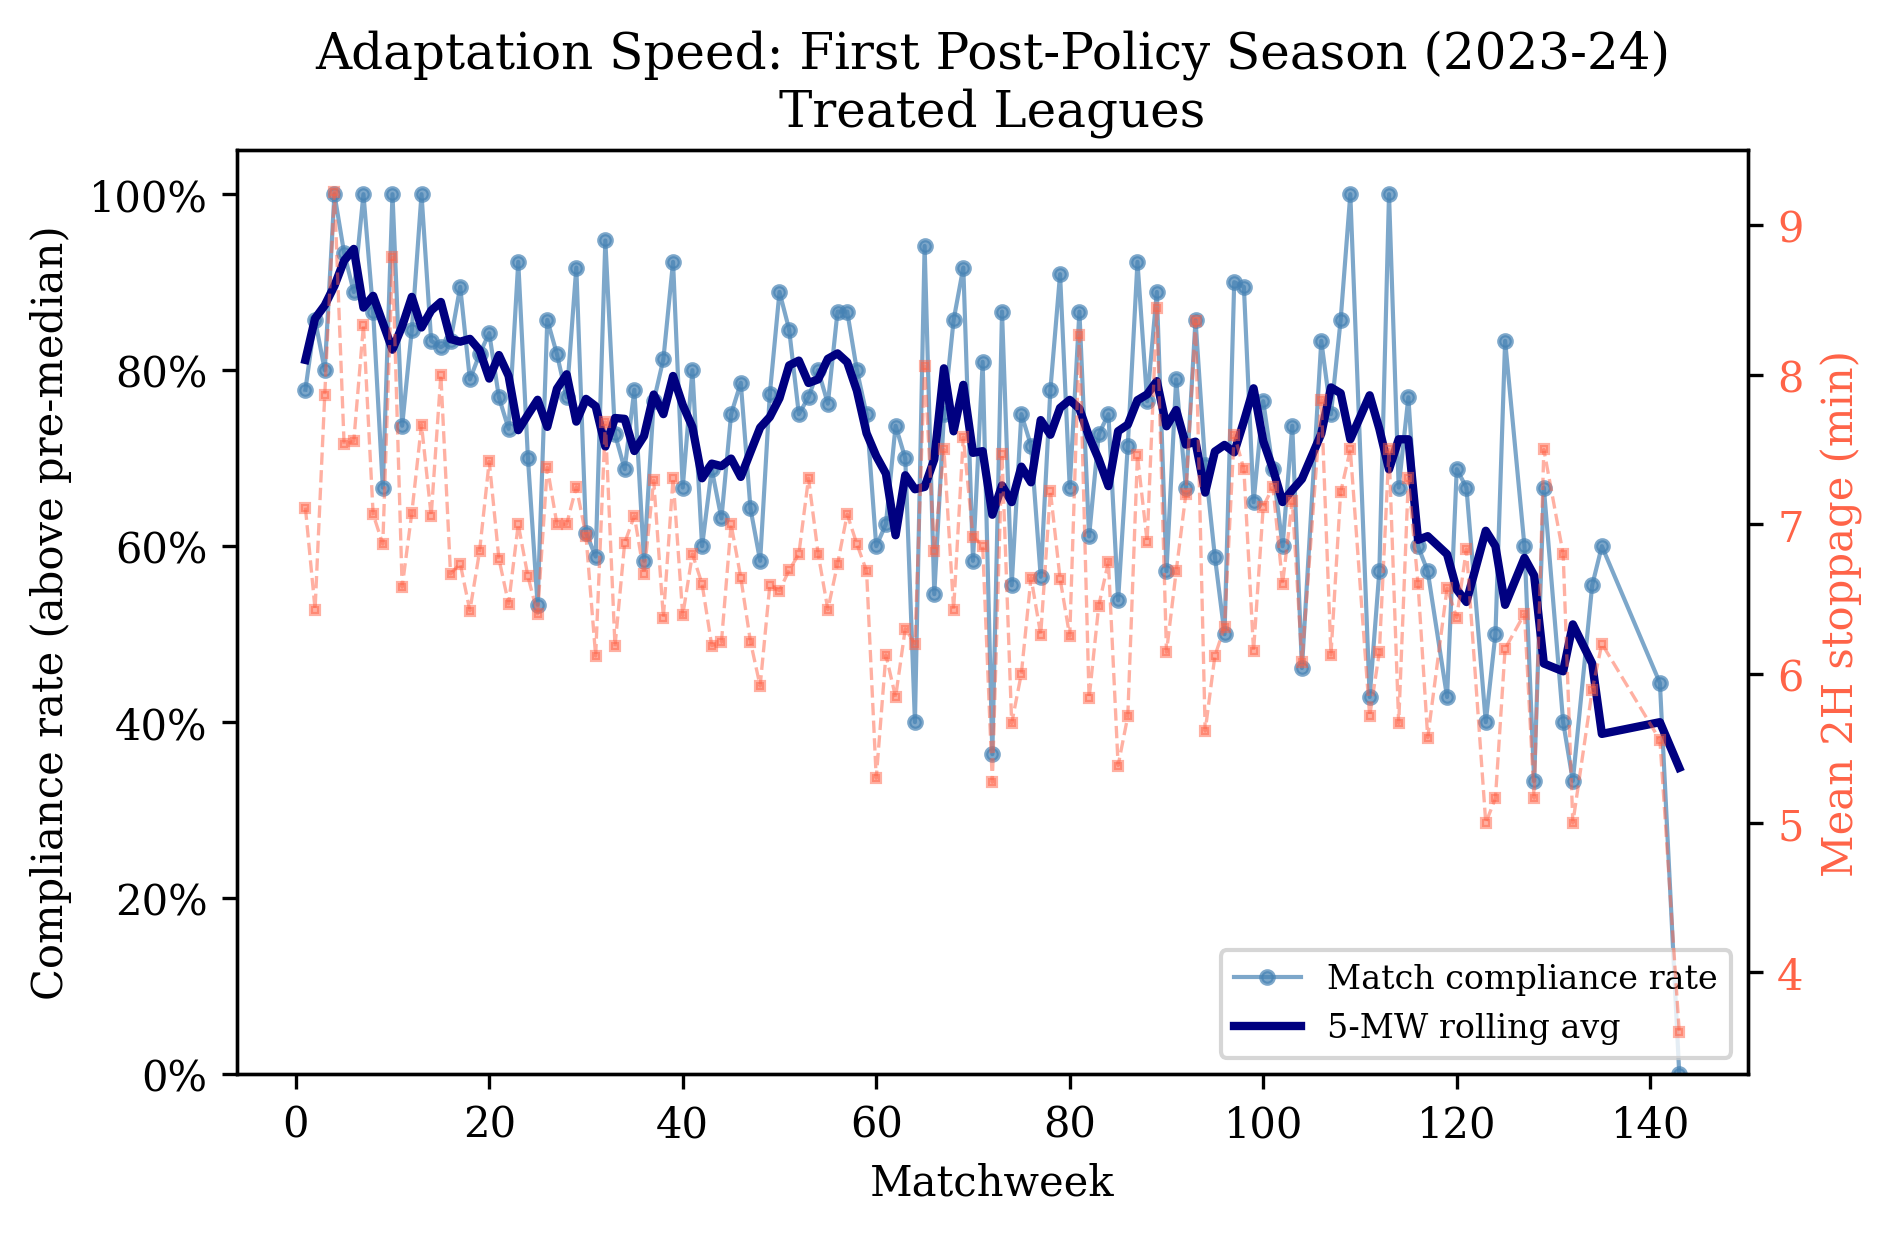
\includegraphics[width=0.8\textwidth]{fig_adaptation_speed_v3}
\caption{Referee compliance rate by matchweek in the 2023--24 season (first post-directive season). Compliance was high from matchweek~1, with no evidence of a gradual learning curve.}
\label{fig:adaptation}
\end{figure}


% ══════════════════════════════════════════════════════════════
%  ON-PITCH EFFECTS
% ══════════════════════════════════════════════════════════════
\section{How the Game Changed: On-Pitch Effects}
\label{sec:onpitch}

With the first stage established (Section~\ref{sec:firststage}) and the compliance mechanism documented (Section~\ref{sec:compliance}), we turn to the central question: what happened on the pitch?\footnote{This section and Sections~\ref{sec:betting}--\ref{sec:welfare} test multiple outcomes. Our three pre-specified primary outcomes are second-half stoppage time (first stage), total goals per match, and goals after the 90th minute. All other on-pitch, betting, and health outcomes are exploratory. We report unadjusted $p$-values throughout; readers should apply multiple-comparison caution to exploratory results.} Total goals were unchanged. The per-minute intensity of play declined. The directive's signature effect was not the creation of new competitive action but its \emph{redistribution} toward the end of matches.

\subsection{Goals: Displacement, Not Creation}
\label{subsec:goals}

We begin with the most closely watched outcome. Table~\ref{tab:onpitch_effects_v3} reports the difference-in-differences estimate for total goals per match. The point estimate is $\hat{\beta} = -0.033$ (SE $= 0.038$, $p = 0.39$, $N = 45{,}433$): a precise zero.\footnote{The total-goals regression uses $N = 45{,}433$: goals are available for more matches than stoppage time. The gap between this and the full panel ($N = 53{,}429$) reflects leagues and seasons with incomplete covariate coverage. The first-stage estimate uses the smaller sample ($N = 36{,}267$) restricted to matches with non-missing stoppage time. Results are qualitatively identical when estimated on the stoppage-time sample.} Pre-directive, matches in this larger sample averaged 2.649 total goals (slightly below the 2.76 reported in Table~\ref{tab:summary_stats_v3}, which conditions on the stoppage-time subsample); post-directive, 2.775. The raw increase of 0.126 goals is fully explained by secular trends common to treated and control leagues, leaving no residual treatment effect.

This null is well-powered. With $N = 45{,}433$ and SE $= 0.038$, our design can detect an increase of 0.11 goals per match (4\% of the pre-treatment mean) at 80\% power. Moreover, the mechanical prediction from the quantity-intensity decomposition (Section~\ref{subsec:decomposition}) is that 1.56 additional minutes at the pre-treatment scoring rate should produce $+0.044$ additional goals per match. The DiD estimate of $-0.033$ is significantly below this mechanical prediction ($t = (-0.033 - 0.044)/0.038 = -2.03$, $p = 0.042$): we can reject not only the null of no effect, but also the null of a purely mechanical increase. The offset is near-complete, and the data are inconsistent with a simple ``more time, more goals'' model.

The null on total goals coexists with a highly significant increase in \emph{late} goals. In a pre-post comparison within treated leagues, goals scored after the 90th minute rose by 0.030 per match ($\text{SE} = 0.007$, $p < 0.001$), from a pre-directive mean of 0.153 to a post-directive mean of 0.183. The juxtaposition of these two results---stable totals, more late goals---defines the central narrative of this section. The directive did not \emph{create} additional goals; it \emph{displaced} them. Scoring opportunities that would have materialized in the final minutes of regular time were, in effect, redistributed into stoppage time. The match as a productive unit generated the same output; only the timing of that output changed (Figure~\ref{fig:goaltiming}).

\begin{figure}[H]
\centering
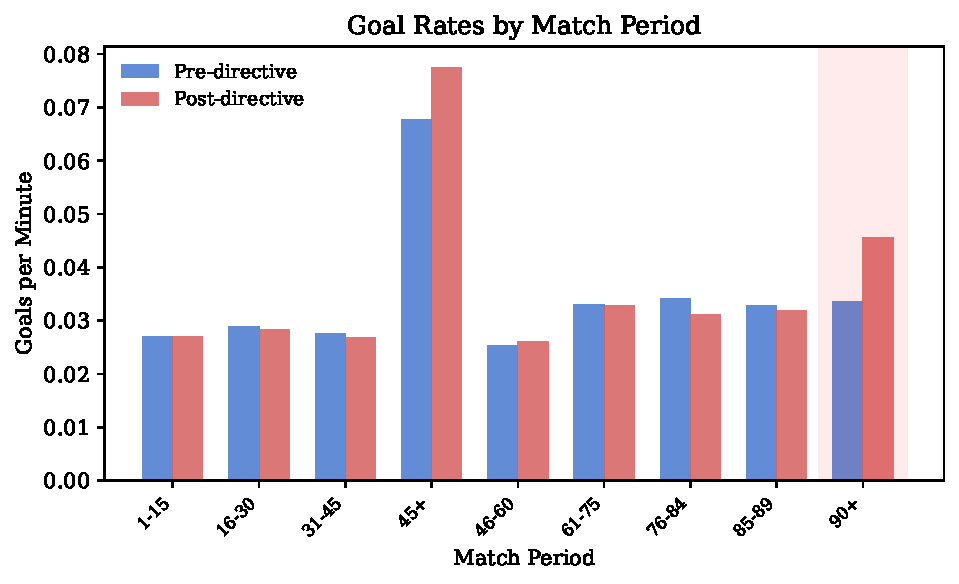
\includegraphics[width=\textwidth]{fig_goal_timing_v3}
\caption{Goals per match by time bin, Big Five leagues, pre- vs.\ post-directive. The post-directive period shows more goals after the 90th minute and fewer in the 76--85 window, consistent with displacement rather than creation.}
\label{fig:goaltiming}
\end{figure}


\subsection{The Quantity--Intensity Decomposition}
\label{subsec:decomposition}

To formalize the displacement result, we decompose the change in each match-level outcome into two channels. Let $Y$ denote an outcome (goals, fouls, cards) observed over an entire match. We can write $Y = r \times T$, where $r$ is the per-minute rate and $T$ is effective playing time. The observed change in $Y$ between regimes can be decomposed as:
\begin{equation}
\label{eq:decomposition}
    \Delta Y = \underbrace{r_{\text{pre}} \cdot \Delta T}_{\text{quantity effect}} + \underbrace{\Delta r \cdot T_{\text{post}}}_{\text{intensity effect}}
\end{equation}
where the \emph{quantity effect} measures how much of the change in $Y$ is attributable to more playing time at the pre-treatment per-minute rate, and the \emph{intensity effect} captures any change in the per-minute rate itself. This is an accounting decomposition, not a causal identification.\footnote{The exact identity is $\Delta Y = r_{\text{pre}} \cdot \Delta T + \Delta r \cdot T_{\text{pre}} + \Delta r \cdot \Delta T$. Our formulation assigns the interaction term ($\Delta r \cdot \Delta T$) to the intensity effect through the choice of post-period weights on the second term. The qualitative conclusions are unchanged under pre-period weighting.} It describes which margin absorbed the change but does not identify \emph{why} the intensity margin moved. We address behavioral interpretations below.

\paragraph{Goals after 90 minutes.} The per-minute scoring rate in stoppage time was 0.029 goals per minute before the directive and 0.029 after ($t = 0.41$, $p = 0.68$)---statistically and substantively unchanged. The raw pre-post change in treated leagues is 0.053 goals per match in the post-90th-minute window (larger than the DiD estimate of 0.030 because the decomposition operates on the treated group alone, whereas the DiD adjusts for control-group trends). This raw change decomposes as 87\% quantity effect (more minutes at the same rate) and 13\% intensity residual, with the intensity component not significantly different from zero. This is the purest form of displacement: the directive purchased additional minutes, and those minutes produced goals at exactly the historical rate. Applied to the DiD estimate instead ($+0.030$), the quantity share would exceed 100\% ($0.046/0.030 = 153\%$), implying a \emph{negative} intensity residual---i.e., the per-minute rate in stoppage time declined slightly relative to control leagues. We report the within-treated decomposition as our primary result because the quantity-intensity framework is an accounting exercise on a single group, not a causal estimator, and the within-group version avoids imposing the DiD's identifying assumption on a descriptive decomposition.

\paragraph{Total goals.} The per-match-minute scoring rate was 0.028 goals per minute before the directive and 0.028 after ($t = 0.73$, $p = 0.47$)---unchanged. The observed raw increase in total goals within treated leagues ($+0.065$ per match) decomposes as 69\% quantity effect (more minutes at the same rate, expected $+0.044$) and 31\% intensity residual ($+0.020$, bootstrap 95\% CI $[-0.037, +0.078]$). The intensity component is not significantly different from zero, confirming that the per-minute scoring rate did not change with the directive. This result complements the DiD null ($\hat{\beta} = -0.033$, $p = 0.39$): after accounting for control-group trends, the small raw increase in treated leagues disappears entirely.

\paragraph{Total fouls.} The foul decomposition reveals a striking pattern. The per-match-minute foul rate \emph{declined significantly} from 0.254 to 0.237 ($t = 15.9$, $p < 0.001$). The mechanical quantity effect of 1.6 additional minutes would predict an \emph{increase} of 0.40 fouls; instead, fouls fell by 0.99 per match. The behavioral intensity residual is $-1.39$ fouls (bootstrap 95\% CI: $[-1.59, -1.19]$)---more than three times larger than the mechanical increase. This intensity decline is consistent with behavioral adaptation: teams foul less frequently per minute of play in the post-directive era.

However, this within-treated-group result must be interpreted alongside the DiD evidence. The DiD coefficient for total fouls is \emph{positive} ($+1.244$, $p < 0.001$; Table~\ref{tab:onpitch_effects_v3}), indicating that control leagues experienced an even larger secular decline. The foul-rate drop in treated leagues therefore reflects a league-wide trend rather than a treatment-specific behavioral response. The decomposition identifies a genuine change in fouling intensity across treated leagues, but the DiD attributes this change to period effects common to all leagues rather than to the directive itself.

\paragraph{Yellow cards.} Yellow cards show a near-zero net change ($+0.014$ per match) masking offsetting components: a mechanical increase of $+0.065$ expected from more playing time, offset by a behavioral residual of $-0.051$. The per-minute yellow card rate declined modestly (0.042 to 0.041, $p = 0.009$). The quantity share (461\%) is uninformative because dividing a non-trivial numerator ($+0.065$) by a near-zero observed change ($+0.014$) inflates the ratio; the individual components are the relevant quantities.

\paragraph{Summary.} Table~\ref{tab:decomposition_v3} collects the decomposition results. For full-match outcomes, the per-minute rate uses total match minutes ($90 + \text{stoppage}_{1H} + \text{stoppage}_{2H}$); for goals after 90', it uses second-half stoppage minutes.\footnote{This denominator choice aligns each outcome with its relevant time base. Goals after 90' are produced during stoppage time; total goals, fouls, and cards accumulate across the entire match.} Two results stand out. First, the per-minute scoring rate---both in stoppage time and across the full match---was unchanged, confirming displacement as the dominant mechanism. Second, the per-minute foul rate dropped significantly, but the DiD attributes this to secular trends rather than the directive ($\hat{\beta}_{\text{fouls}} = +1.244$, $p < 0.001$). Figure~\ref{fig:decomposition_v3} in Appendix~\ref{app:figures} provides a visual decomposition.

\begin{table}[htbp]
\centering
\caption{Quantity--Intensity Decomposition}
\label{tab:decomposition_v3}
\begin{threeparttable}
\begin{tabular}{lcccccc}
\toprule
Outcome & $\Delta$ Stoppage & Observed $\Delta$ & Quantity & Intensity & Qty Share & Rate $p$ \\
\midrule
  Total goals & +1.56 & +0.065 & +0.044 & +0.020 & 69\% & 0.468 \\
  Total fouls & +1.56 & -0.990 & +0.396 & -1.387 & $-$40\% & 0.000*** \\
  Yellow cards & +1.56 & +0.014 & +0.065 & -0.051 & 461\% & 0.009** \\
  Goals after 90' & +1.56 & +0.053 & +0.046 & +0.007 & 87\% & 0.685 \\
\bottomrule
\end{tabular}
\begin{tablenotes}[flushleft]\footnotesize
\item \textit{Notes:} Quantity channel = $\Delta$stoppage $\times$ pre-treatment per-minute rate. Intensity = observed $-$ expected. Bootstrap 95\% CIs (1,000 iterations). Rate $p$-value from Welch $t$-test of per-minute rates pre vs.\ post. For full-match outcomes (total goals, fouls, cards), the per-minute rate uses total match minutes ($90 + \text{stoppage}_{1H} + \text{stoppage}_{2H}$) as the denominator. For goals after 90', the rate uses second-half stoppage minutes only. Negative quantity shares arise when the quantity and observed changes have opposite signs.
\end{tablenotes}
\end{threeparttable}
\end{table}



\subsection{Game-Changing Goals: When Results Hang in the Balance}
\label{subsec:game_changing}

The displacement of goals toward the end of matches increases the frequency of \emph{game-changing goals}---goals scored after the 85th minute that alter the match result.

The pre-post estimate for game-changing goals after minute 85 is $\hat{\beta} = 0.035$ ($\text{SE} = 0.007$, $p < 0.001$).\footnote{Because minute-level data are available only for Big Five leagues and the Championship, this estimate uses a pre-post comparison within treated leagues with league and season fixed effects, not the full DiD. The smaller sample ($N = 14{,}441$) precludes a treated-vs-control design for this outcome.} Pre-directive, 17.9\% of matches featured at least one such goal; post-directive, the share rose to 21.4\%---an increase of approximately 20\%.

This effect is economically significant. From the perspective of a broadcaster, a late game-changing goal is among the highest-value events in a football match: it sustains audience engagement through the final minutes and generates highlights that drive post-match media consumption. From the perspective of a fan, it is the difference between a match that is ``over'' at minute 80 and one that remains alive until the final whistle.

Importantly, the increase in game-changing goals is a \emph{redistribution} effect, not a creation effect. Because total goals did not change, the additional late goals that altered results came at the expense of goals that would have been scored earlier. The directive did not make football more ``productive'' in terms of total goals; it made football more \emph{dramatic} by increasing the probability that the decisive moment occurs late (Figure~\ref{fig:result_changes_v3} in Appendix~\ref{app:figures}).


\subsection{Distributional Effects}
\label{subsec:distributional}

We now examine the full distribution of stoppage time using quantile treatment effects (QTEs).

\begin{figure}[htbp]
\centering
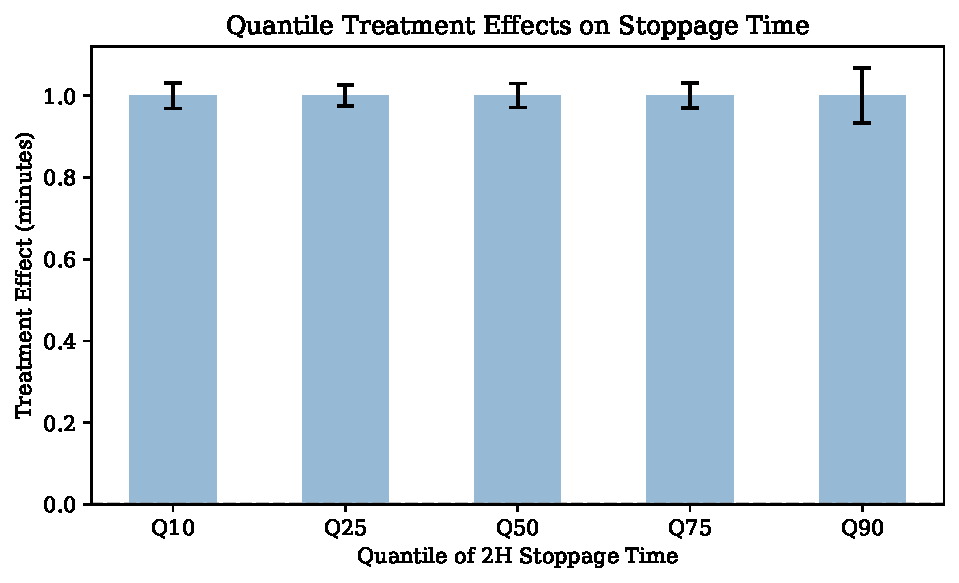
\includegraphics[width=\textwidth]{fig_quantile_effects_v3}
\caption{Quantile treatment effects on second-half stoppage time. Each point shows the estimated DiD effect at a given percentile of the stoppage-time distribution. The effect is approximately 1.0 minute at every quantile, indicating a pure location shift rather than a change in the distribution's shape.}
\label{fig:quantile_effects_v3}
\end{figure}

Figure~\ref{fig:quantile_effects_v3} displays the estimated treatment effect at the 10th, 25th, 50th, 75th, and 90th percentiles of the stoppage-time distribution. The effect is strikingly uniform: approximately 1.0 minute at every quantile. The \emph{entire} distribution shifted rightward by approximately one minute, preserving its shape.

This uniformity rules out a model in which the directive primarily affected the tails---for example, by eliminating very short stoppages or creating very long ones while leaving the middle of the distribution unchanged. The directive was, in distributional terms, a pure location shift.

Despite the uniform shift in quantiles, the directive had asymmetric effects on the probability of extreme stoppages, a mechanical consequence of the nonlinear relationship between a location shift and tail probabilities. The probability that stoppage time exceeded 8 minutes rose from 7.1\% to 27.8\% in treated leagues---a DiD coefficient of $0.087$---transforming what had been a roughly one-in-fourteen event into a one-in-four event. The probability of exceeding 10 minutes rose from 1.8\% to 9.2\%, a fivefold increase from a low base.


\subsection{Competitive Balance}
\label{subsec:competitive_balance}

A natural concern is that the redistribution of goals toward the end of matches might systematically advantage certain types of teams. We test for changes in competitive balance using the standard deviation of final league points and the normalized Herfindahl--Hirschman Index (NHHI) of points concentration. Neither measure shows a statistically significant change following the directive ($\hat{\beta}_{\text{SD}} = 0.17$, SE $= 0.68$, $p = 0.80$; $\hat{\beta}_{\text{NHHI}} = 0.0007$, SE $= 0.0005$, $p = 0.14$; $N = 138$ league-seasons). The test has 80\% power to detect a change of 1.9 points in the standard deviation of league points (12.4\% of the pre-directive mean of 15.5), sufficient to rule out large disruptions but not subtle rebalancing.

The null is consistent with the displacement interpretation. If the directive redistributed goals \emph{across time within matches} without changing total goals, and if the redistribution was not systematically correlated with team quality, then league-level competitive balance should be unaffected (Figure~\ref{fig:competitive_balance_v3} in Appendix~\ref{app:figures}).


\subsection{Heterogeneous Effects by Game State}
\label{subsec:het_game_state}

A large literature documents that referees respond to the competitive context of a match. \citet{garicano2005favoritism} found that La~Liga referees added more stoppage time when the home team was behind; \citet{dohmen2008professionals} and \citet{bekes2024favoritism} documented similar patterns in other leagues. If the directive amplified rather than replaced this strategic behavior, the treatment effect should vary with the half-time score. We test this by estimating separate DiD regressions conditional on the half-time game state: tied, home leading, or away leading.

\begin{table}[htbp]
\centering
\caption{Heterogeneous Treatment Effects by Half-Time Game State}
\label{tab:het_game_state}
\begin{threeparttable}
\begin{tabular}{lccccc}
\toprule
Game state & $\hat{\beta}$ & SE & $p$ & 95\% CI & $N$ \\
\midrule
  Tied & 0.724* & (0.309) & 0.019 & [0.119, 1.329] & 15,292 \\
  Home leading & 0.849*** & (0.236) & 0.000 & [0.386, 1.312] & 11,945 \\
  Away leading & 0.626* & (0.313) & 0.045 & [0.013, 1.239] & 9,029 \\
  Close ($\leq$1 goal) & 0.740** & (0.286) & 0.010 & [0.180, 1.301] & 30,915 \\
  Decided ($\geq$2 goals) & 0.741* & (0.297) & 0.013 & [0.159, 1.324] & 5,351 \\
\midrule
  Tied $\times$ Treatment & 0.121 & (0.092) & 0.191 & & \\
\bottomrule
\end{tabular}
\begin{tablenotes}[flushleft]\footnotesize
\item \textit{Notes:} Each row reports a separate DiD regression of 2H stoppage time on Post $\times$ Treated, with league and season fixed effects, clustering at the league level. Game state is determined by the half-time score. The interaction tests whether the treatment effect differs significantly for tied matches. $^{*}p<0.05$, $^{**}p<0.01$, $^{***}p<0.001$.
\end{tablenotes}
\end{threeparttable}
\end{table}


The treatment effect is remarkably uniform across game states (Table~\ref{tab:het_game_state}). Matches tied at half-time show a treatment effect of $0.724$ minutes (SE $= 0.309$), while matches with the home team leading show $0.849$ (SE $= 0.236$) and matches with the away team leading show $0.626$ (SE $= 0.313$). A formal interaction test of the tied$\times$treatment coefficient is insignificant ($\beta = 0.121$, $p = 0.191$). The effect is also indistinguishable between close games ($\leq 1$ goal margin: $\beta = 0.740$) and decided games ($\geq 2$ goal margin: $\beta = 0.741$).

This uniformity contrasts sharply with the referee bias documented by \citet{garicano2005favoritism} and \citet{dohmen2008professionals}, where stoppage time varied systematically with game state. The null on heterogeneity supports the directive's stated purpose: mechanical enforcement of existing rules, not a behavioral intervention. The directive appears to have shifted referees from a strategic mode---in which stoppage time responded to social pressure and competitive context---to a bureaucratic compliance mode in which time is added uniformly regardless of the score.


\subsection{Summary of On-Pitch Effects}

\begin{table}[htbp]
\centering
\caption{On-Pitch Effects of the Stoppage-Time Directive}
\label{tab:onpitch_effects_v3}
\small
\begin{threeparttable}
\begin{tabular}{lccccc}
\toprule
 & $\hat{\beta}$ & SE & Pre-mean & Post-mean & N \\
\midrule
\multicolumn{6}{l}{\textit{Panel A: Goal Effects}} \\
  Goals in 90+ min & +0.0302*** & (0.0069) & 0.153 & 0.183 & 16,212 \\
  Result changed in stoppage & +0.0303*** & (0.0053) & 0.073 & 0.103 & 14,441 \\
  Late equalizer & +0.0120** & (0.0044) & 0.053 & 0.065 & 14,441 \\
  Late winner & +0.0126* & (0.0050) & 0.075 & 0.088 & 14,441 \\
  Total goals per match & -0.0328 & (0.0379) & 2.649 & 2.775 & 45,433 \\
\midrule
\multicolumn{6}{l}{\textit{Panel B: Result Distribution}} \\
  Draw rate & +0.0026 & (0.0100) & 0.264 & 0.261 & 45,433 \\
  Home win rate & -0.0079 & (0.0114) & 0.436 & 0.432 & 45,433 \\
  Away win rate & +0.0054 & (0.0106) & 0.300 & 0.307 & 45,433 \\
\midrule
\multicolumn{6}{l}{\textit{Panel C: Fouls and Cards}} \\
  Total fouls & +1.2441*** & (0.1298) & 25.757 & 24.020 & 39,130 \\
  Total cards & -0.0531 & (0.0516) & 4.269 & 4.307 & 40,469 \\
  Home yellow cards & -0.0530 & (0.0308) & 1.904 & 1.912 & 40,469 \\
  Away yellow cards & -0.0199 & (0.0324) & 2.157 & 2.203 & 40,469 \\
  Home red cards & +0.0091 & (0.0069) & 0.092 & 0.089 & 40,469 \\
  Away red cards & +0.0106 & (0.0074) & 0.116 & 0.104 & 40,469 \\
\midrule
\multicolumn{6}{l}{\textit{Panel D: Competitive Balance}} \\
  SD of points & +0.1717 & (0.6848) & 15.476 & 15.469 & 138 \\
  Normalized HHI & +0.0007 & (0.0005) & 0.006 & 0.006 & 138 \\
\bottomrule
\end{tabular}
\begin{tablenotes}
\small
\item Notes: OLS regressions with league and season FE. HC1 robust SEs in parentheses (the first-stage specification in Table~\ref{tab:first_stage} uses league-clustered SEs; qualitative conclusions are unchanged).
$^{***}p<0.001$, $^{**}p<0.01$, $^{*}p<0.05$.
Total goals and Panels B--D use match-level DiD (treated vs control leagues).
Goals in 90+ min, result changed in stoppage, late equalizer, and late winner use pre-post comparisons within treated leagues with minute-level data.
Panel D uses league-season level DiD.
\end{tablenotes}
\end{threeparttable}
\end{table}

The directive changed the temporal distribution of goals without changing their total quantity, did not reduce fouls relative to control leagues (the DiD coefficient is positive), and left match outcomes---draws, home wins, away wins---unchanged. The game got longer and late drama became more common, but the competitive equilibrium was preserved.


% ══════════════════════════════════════════════════════════════
%  BETTING MARKETS
% ══════════════════════════════════════════════════════════════
\section{Betting Markets and the Regime Change}
\label{sec:betting}

Sports betting markets offer a high-frequency laboratory for studying how
prices respond to regulatory change. The FIFA directive altered the temporal
structure of matches---extending second-half stoppage time by approximately
1.6 minutes on average in the most-treated leagues---but left the fundamental
object of most wagers, total goals, essentially unchanged. This section asks
whether sophisticated and retail betting markets distinguished between these
two facts.

\subsection{Overall Forecast Accuracy}
\label{subsec:brier}

We evaluate forecast accuracy using Brier scores for match-outcome (1X2)
and over/under markets, estimating difference-in-differences specifications
of the form used throughout the paper. If the directive degraded
bookmakers' ability to forecast outcomes, we would observe a positive shift
in Brier scores (worse calibration) in the post-directive period for
treated leagues relative to controls.

Table~\ref{tab:betting_efficiency_v3} reports the results. For Pinnacle, widely regarded
as the sharpest global bookmaker, the Brier-score DiD estimate is $+0.007$
(SE~$= 0.008$, $p = 0.41$, $N = 27{,}867$). For Bet365, the
largest retail sportsbook by volume, the estimate is $+0.005$
(SE~$= 0.008$, $p = 0.58$, $N = 28{,}382$). Estimates for the
remaining bookmakers in our sample---bwin, Interwetten, William Hill,
and bet-at-home---are of similar magnitude and similarly insignificant.
Across the full panel, there is no evidence that the directive impaired
forecast accuracy for any bookmaker.

\begin{table}[htbp]
\centering
\caption{Betting Market Efficiency: DiD Estimates}
\label{tab:betting_efficiency_v3}
\small
\begin{threeparttable}
\begin{tabular}{lccccc}
\toprule
Outcome & $\hat{\beta}$ & SE & $p$-value & $N$ & Tier \\
\midrule
\multicolumn{6}{l}{\textit{Panel A: Brier Score Accuracy}} \\
\quad Pinnacle & $+0.0069$ & $0.0084$ & $0.4098$ & $27,867$ & sharp \\
\quad Bet365 & $+0.0045$ & $0.0081$ & $0.5750$ & $28,382$ & retail \\
\quad bwin & $+0.0047$ & $0.0084$ & $0.5818$ & $27,105$ & retail \\
\quad Interwetten & $+0.0066$ & $0.0156$ & $0.6710$ & $21,386$ & retail \\
\quad William Hill & $+0.0091$ & $0.0093$ & $0.3283$ & $25,571$ & retail \\
\quad bet-at-home & $+0.0087$ & $0.0119$ & $0.4651$ & $23,061$ & retail \\
\quad Sharp average & $+0.0069$ & $0.0084$ & $0.4098$ & $27,867$ & sharp \\
\quad Retail average & $+0.0047$ & $0.0080$ & $0.5606$ & $28,402$ & retail \\
\midrule
\multicolumn{6}{l}{\textit{Panel B: Placebo \& Positive Controls}} \\
\quad 1H total goals & $-0.0234$ & $0.0240$ & $0.3307$ & $53,397$ & placebo \\
\quad 1H stoppage time & $+0.5496^{***}$ & $0.0464$ & $0.0000$ & $29,317$ & placebo \\
\quad 2H total goals & $-0.0012$ & $0.0262$ & $0.9648$ & $53,396$ & control \\
\quad 2H stoppage time & $+0.7471^{***}$ & $0.0514$ & $0.0000$ & $36,413$ & control \\
\midrule
\multicolumn{6}{l}{\textit{Panel C: Market Structure}} \\
\quad O/U line level & $-0.0737$ & $0.0398$ & $0.0643$ & $967$ & \\
\quad CLV 1X2 home & $+0.0215$ & $0.0128$ & $0.0920$ & $21,793$ & \\
\quad CLV O/U over & $+0.0059$ & $0.0034$ & $0.0817$ & $21,791$ & \\
\quad CLV Pinnacle O/U & $+0.0018$ & $0.0034$ & $0.6018$ & $21,233$ & \\
\bottomrule
\end{tabular}
\begin{tablenotes}
\small
\item \textit{Notes:} All regressions include league and season fixed effects.
HC1 robust standard errors. $^{*}p<0.05$, $^{**}p<0.01$, $^{***}p<0.001$.
Panel B: 1H outcomes are null-expected placebos; 2H outcomes are positive-expected controls.
\end{tablenotes}
\end{threeparttable}
\end{table}


Two complementary explanations are consistent with this null result.
First, markets may have rapidly incorporated the regime change, adjusting
lines within the opening weeks of the post-directive period such that
forecast accuracy was restored before it could register in
season-level comparisons. Second---and more parsimoniously---the directive
may not have changed the object being forecasted. Since total goals per
match remained stable (Section~\ref{subsec:goals}), the over/under lines that
bookmakers set before kickoff required little revision: the same number of
goals was scored, merely redistributed across the ninety-plus minutes.
Both explanations imply well-functioning markets; they differ only in
whether there was anything to which markets needed to adjust. This contrasts with
\citet{fischer2022home}, who found that COVID-era ``ghost games'' produced
temporary betting market inefficiency as odds were slow to adjust to the
diminished home advantage---a setting where the underlying outcome distribution
\emph{did} change.

\subsection{Bookmaker Disagreement and Market Segmentation}
\label{subsec:disagreement}

A standard prediction of models with heterogeneous information is that
less-informed agents adjust more slowly to structural breaks, producing
transient disagreement between ``sharp'' (professional, low-margin) and
``soft'' (retail, higher-margin) bookmakers \citep{levitt2004gambling}. If the
directive constituted a genuine informational shock, we would expect
Pinnacle's forecasts to dominate Bet365's in the immediate
post-directive period, with the gap narrowing over time.

We find no evidence of such a pattern. The difference in Brier-score DiD
between the sharp-bookmaker average ($+0.007$) and the retail-bookmaker average ($+0.005$) is
$+0.002$ ($z = 0.19$, $p = 0.85$, assuming independence across market segments)---economically negligible and statistically insignificant. Both market
segments absorbed the regime change---or its irrelevance to total
goals---symmetrically. This null is informative: it suggests that the
directive did not generate the kind of private-information advantage that
separates sharp from retail books in other settings, such as injury news
or lineup changes \citep{croxsonreade2014} (Figure~\ref{fig:odds_spread_v3} in Appendix~\ref{app:figures}).

\subsection{Speed of Adjustment}
\label{subsec:halflife}

To characterize the dynamics of any market response, we estimate the
``half-life'' of excess miscalibration following the directive. We fit
exponential-decay models to the week-by-week Brier-score residuals in
both the 1X2 and over/under markets, asking how quickly any initial
deterioration in accuracy dissipated.

The exercise yields a stark result: for the 1X2 market, the exponential
fit fails entirely because there is no detectable initial excess to
decay. For the over/under market, the same pattern holds---there is no
positive excess in the opening weeks from which a decay trajectory could
be estimated. The most straightforward interpretation is that markets
adjusted so quickly that no measurable adjustment period existed at the
matchweek frequency, or---consistent with the parsimonious explanation
offered above---that there was no adjustment to make.

This finding is consistent with the efficient markets hypothesis: the
directive was publicly announced, universally applied, and easily
observable in real time, lacking the ambiguity that characterizes settings
where markets adjust slowly (Figure~\ref{fig:bookmaker_adjustment_v3} in Appendix~\ref{app:figures}).
The directive changed \emph{when} goals occurred but not \emph{how many}---and
over/under lines, the most directly affected product, showed no
systematic miscalibration at any horizon.

\subsection{Closing-Line Value}
\label{subsec:clv}

Closing-line value (CLV) measures whether late-arriving information
systematically moves odds in one direction, providing a test of whether
informed bettors exploited knowledge of the directive's implications.
We regress the closing-line drift (the change in
implied probability between opening and closing lines) on a
post-directive indicator, controlling for league and season fixed effects.

For the 1X2 home-win market, the post-directive coefficient is $0.021$
($p = 0.092$). For the over/under ``over'' market, the coefficient is
$0.006$ ($p = 0.082$). Neither estimate is significant at conventional
levels, though both are marginally suggestive of slight late-market
learning---a pattern consistent with a small number of sophisticated
bettors incorporating match-specific stoppage-time expectations into
their models. Notably, the Pinnacle over/under closing-line drift
coefficient is $0.002$ ($p = 0.60$), indicating that the sharpest
benchmark in our sample exhibited no systematic drift whatsoever. The
marginal effects, where they appear, are confined to softer books and are
too small to survive standard multiple-testing corrections.

Taken together, the betting-market evidence tells a consistent story: the directive passed through markets without leaving a measurable trace. No deterioration in forecast accuracy, no differential adjustment between sharp and retail segments, no measurable adjustment period, and no economically significant closing-line drift.\footnote{The over/under line level shows a marginally significant decline of $-0.074$ ($p = 0.064$), but this estimate is based on only 967 observations and should be interpreted cautiously.} The most parsimonious interpretation is that there was little to adjust: the directive changed the temporal distribution of goals but not their total, and over/under lines were priced off the same underlying total that remained stable.


% ══════════════════════════════════════════════════════════════
%  ROBUSTNESS
% ══════════════════════════════════════════════════════════════
\section{Robustness and the Design's Limitations}
\label{sec:robustness}

This section subjects the first-stage result to a battery of robustness exercises. We organize them from strongest to weakest, and we conclude with an honest assessment of what the design can and cannot identify. The exercises are summarized in Table~\ref{tab:robustness_v3}; we discuss each in turn.

\begin{table}[htbp]
\centering
\caption{Robustness Checks: V3 Suite}
\label{tab:robustness_v3}
\begin{threeparttable}
\begin{tabular}{llcccc}
\toprule
Test & Specification & $\hat{\beta}$ & SE & $p$ & $N$ \\
\midrule
\multicolumn{6}{l}{\textit{Panel A: Placebo Tests}} \\
  H1 Placebo & 1H Stoppage & +0.550 & 0.046 & 0.000 & 29,317 \\
  HT Goals & Halftime goals & -0.024 & 0.023 & 0.298 & 55,488 \\
\midrule
\multicolumn{6}{l}{\textit{Panel B: Anticipatory Effects}} \\
  Partial (2022--23) & Three-period DiD & +0.340 & 0.258 & 0.187 & 36,413 \\
  Full (2023--24+) & Three-period DiD & +0.807 & 0.283 & 0.004 & 36,413 \\
\midrule
\multicolumn{6}{l}{\textit{Panel C: Sample Robustness}} \\
  Excl.\ 2022--23 & Baseline DiD & +0.810 & 0.052 & 0.000 & 32,357 \\
  Leave-one-out & Range & [+0.571, +0.961] & --- & --- & --- \\
\midrule
\multicolumn{6}{l}{\textit{Panel D: Permutation Inference}} \\
  Random treatment & 1000 perms & +0.747 & --- & 0.0450 & 1,000 \\
\bottomrule
\end{tabular}
\begin{tablenotes}[flushleft]\footnotesize
\item \textit{Notes:} Panel A reports falsification tests on outcomes unaffected by the FIFA directive. The HT Goals sample ($N = 55{,}488$) includes the S\"{u}per Lig, which has goals data but no stoppage-time data; excluding it does not change the result. Panel B separates anticipatory (2022--23) from full treatment effects. Panel C excludes the transition season; leave-one-out range from Table~\ref{tab:sensitivity}. Panel D reports two-sided permutation $p$-value from random treatment reassignment across leagues.
\end{tablenotes}
\end{threeparttable}
\end{table}



\subsection{Specification Curve}
\label{subsec:spec_curve}

Following \citet{simonsohn2020specification}, we estimate 420 specifications varying six researcher degrees of freedom: the dependent variable (3 levels: 2H stoppage, total stoppage, log-transformed 2H stoppage), fixed effects (3 levels: league only, season only, league $+$ season), clustering (3 levels: HC1, league-clustered, match-level), the sample restriction (5 levels: full, no-COVID, Big Five only, post-2017, clean controls), the post-period definition (2 levels: including or excluding 2022--23), and covariates (2 levels: parsimonious or with controls). The full Cartesian product ($3 \times 3 \times 3 \times 5 \times 2 \times 2 = 540$) is reduced to 420 after excluding specifications that are logically invalid (e.g., Big Five-only sample with league-only fixed effects, which is collinear with the treatment indicator) or lack sufficient data. Each specification is a fully independent estimation.

Figure~\ref{fig:spec_curve_v3} displays the results. The median coefficient across all 420 specifications is $\hat{\beta} = 0.669$. Of the 420 specifications, 88.8\% are statistically significant at the 5\% level and 95.0\% produce positive point estimates. The interquartile range is $[0.44, 0.94]$, comfortably excluding zero.

\begin{figure}[H]
\centering
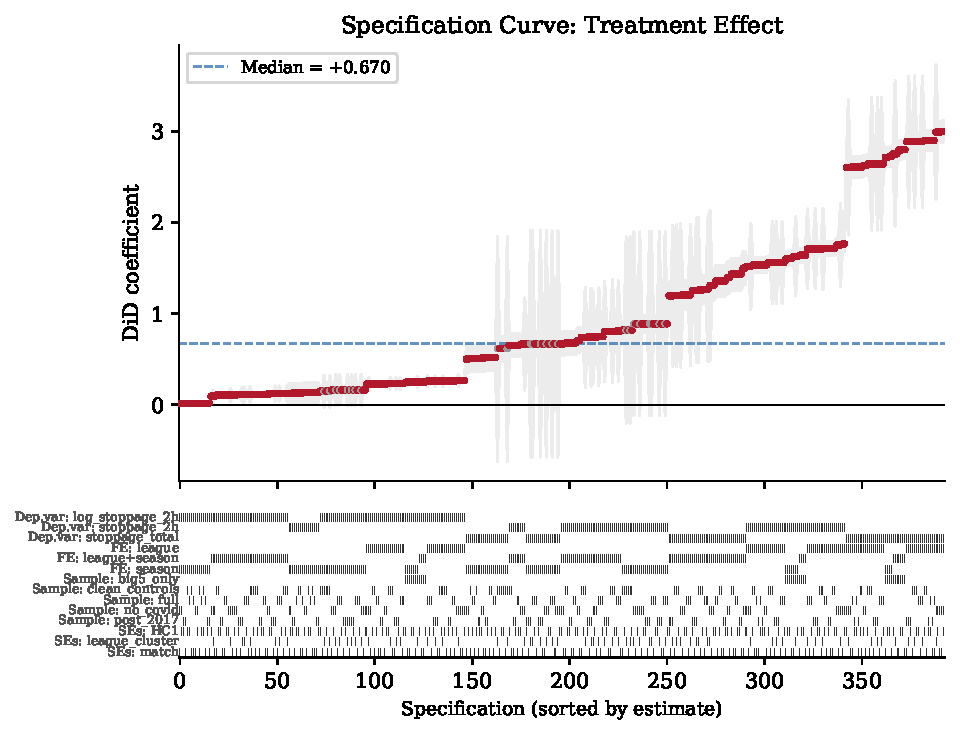
\includegraphics[width=0.85\textwidth]{fig_spec_curve_v3}
\caption{Specification curve analysis: 420 specifications. Each point represents one specification, ordered by point estimate. The shaded band shows the interquartile range.}
\label{fig:spec_curve_v3}
\end{figure}

The specification curve confirms that the first-stage result is not an artifact of a particular specification choice. The sign is stable across 95\% of reasonable analytic decisions, and statistical significance is maintained across 88.8\%. A small number of specifications (27 of 420) with certain fixed-effect and clustering combinations produce numerically unstable estimates due to near-collinearity; these are excluded from Figure~\ref{fig:spec_curve_v3} but are included in the 88.8\% and 95.0\% rates reported above.\footnote{The excluded specifications arise when fixed effects absorb nearly all identifying variation while clustering compresses the effective degrees of freedom, producing near-singular design matrices. Of the 27 excluded specifications, 24 produce significant positive estimates, so their exclusion from the figure does not inflate the significance rate.}


\subsection{Permutation Inference}
\label{subsec:permutation}

Permutation inference provides a design-based test of the sharp null hypothesis that the directive had no effect on any league's stoppage time \citep{anderson2008multiple}. We randomly reassign treatment status across leagues 1,000 times, re-estimating the DiD each time, and compare the observed coefficient to the resulting null distribution (Figure~\ref{fig:permutation_v3}).

\begin{figure}[H]
\centering
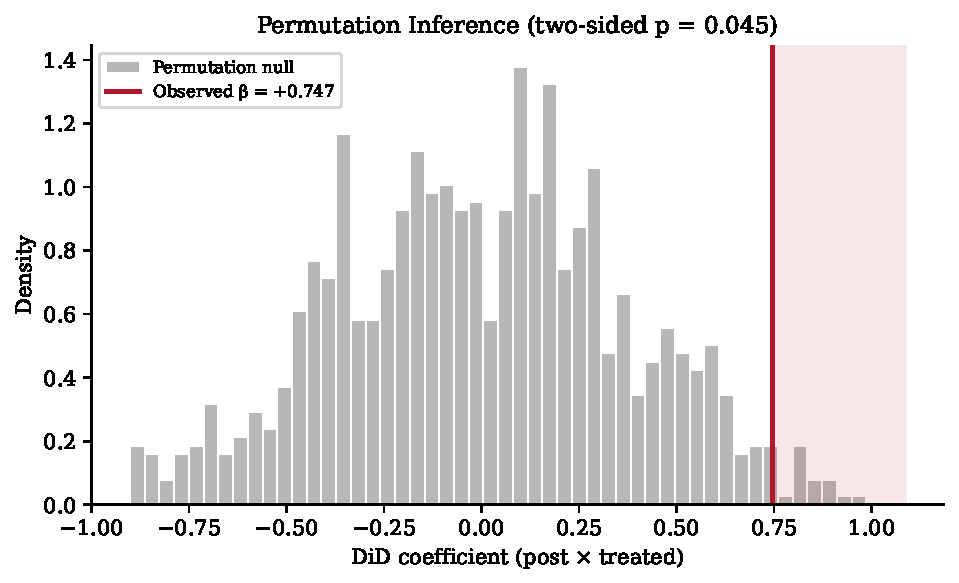
\includegraphics[width=0.75\textwidth]{fig_permutation_v3}
\caption{Permutation inference: distribution of placebo DiD coefficients under 1,000 random treatment reassignments. The vertical dashed line marks the observed coefficient ($\hat{\beta} = 0.747$; the permutation uses a parsimonious specification with $N = 36{,}413$, yielding a coefficient slightly above the primary estimate of $0.744$). The null distribution has mean $-0.002$ and standard deviation $0.371$.}
\label{fig:permutation_v3}
\end{figure}

The null distribution is centered at $-0.002$ with a standard deviation of 0.371. The observed coefficient of 0.747 falls 2.02 standard deviations from the null mean. The two-sided $p$-value is 0.045. Under the sharp null of no treatment effect on any league, the probability of observing a coefficient as extreme as 0.747 by chance is 4.5\%.

This test does not require parallel trends. The permutation distribution accounts for whatever serial correlation, league-specific trends, and heteroskedasticity exist in the data---it simply asks whether the observed estimate is unusual relative to what random treatment assignment would produce.


\subsection{Goodman-Bacon Decomposition}
\label{subsec:goodmanbacon}

The two-way fixed effects (TWFE) estimator is a weighted average of all possible $2 \times 2$ DiD comparisons in the panel \citep{goodmanbacon2021difference, deChaisemartin2020}; see \citet{rothetal2023} for a synthesis of recent advances. Alternative heterogeneity-robust estimators---including the interaction-weighted approach of \citet{sunAbraham2021} and the imputation estimator of \citet{borusyak2024revisiting}---are designed for staggered-adoption settings; our near-simultaneous adoption makes them less necessary, but we report the Goodman-Bacon decomposition as a transparency check. Our setting is relatively clean---all treated leagues adopted the directive within an 8-day window in August 2023---but heterogeneity across leagues could still distort the aggregate.

The decomposition produces 45 pairwise $2 \times 2$ DiD estimates. The weighted average across all pairs is 0.718, close to our primary TWFE estimate of 0.744. This proximity confirms that the TWFE is well-behaved in our setting: near-simultaneous treatment onset means there are no ``forbidden comparisons'' between early and late adopters (Figure~\ref{fig:goodman_bacon_v3}).

\begin{figure}[H]
\centering
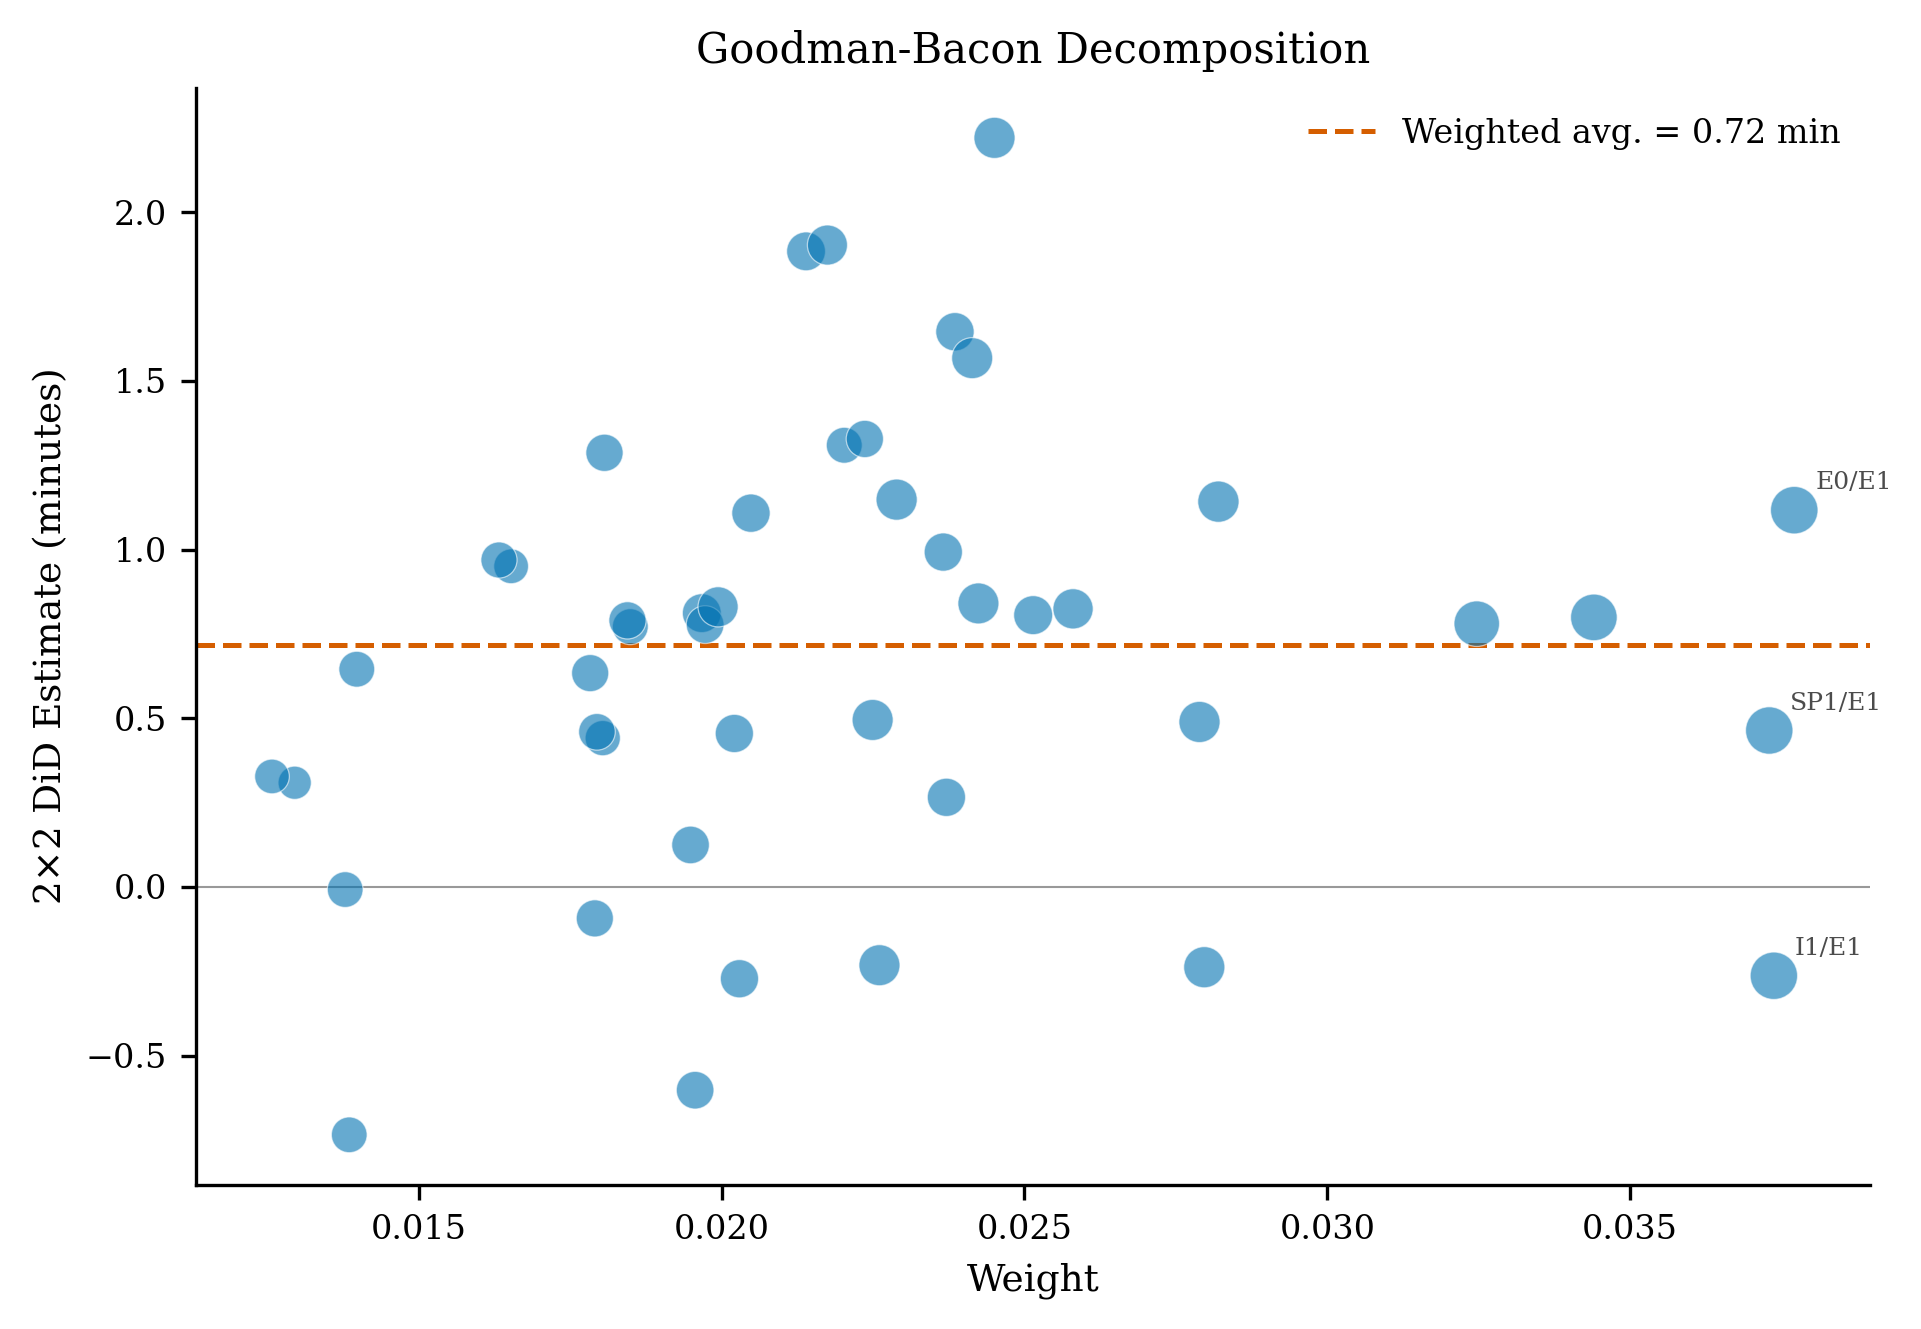
\includegraphics[width=0.85\textwidth]{fig_goodman_bacon_v3}
\caption{Goodman-Bacon decomposition: 45 bilateral $2 \times 2$ DiD estimates. Each point is one league pair; marker size is proportional to weight in the TWFE average. The dashed line marks the TWFE estimate.}
\label{fig:goodman_bacon_v3}
\end{figure}

The decomposition reveals meaningful heterogeneity. The Premier League vs.\ Championship comparison produces the largest weighted bilateral estimate ($+1.117$), while Serie~A comparisons tend to produce negative bilateral estimates, pulling the aggregate downward. The range of bilateral estimates spans $[-0.735, +2.220]$, confirming substantial league-level treatment effect heterogeneity.


\subsection{Leave-One-Out Sensitivity}
\label{subsec:loo}

To assess whether any single league drives the aggregate result, we re-estimate the specification 15 times, each time dropping one league (Table~\ref{tab:sensitivity}). The leave-one-out range is $[0.571, 0.961]$, and all 15 estimates remain statistically significant at the 1\% level.

The largest deviation from baseline occurs when Serie~A is dropped ($\hat{\beta} = 0.961$), consistent with Serie~A's muted enforcement response pulling the pooled estimate downward. Dropping the Premier League---the largest enforcer---reduces the estimate to 0.571 but preserves significance. No single league is indispensable for the result.

\begin{table}[htbp]
\centering
\begin{threeparttable}
\caption{Leave-One-Out Sensitivity of the First-Stage Effect}
\label{tab:sensitivity}
\begin{tabular}{lccccr}
\toprule
Dropped league & $\hat{\beta}$ & SE & $p$ & $N$ & $\Delta\hat{\beta}$ \\
\midrule
\multicolumn{6}{l}{\textit{Panel A: Drop one control league}} \\[3pt]
Belgian First Division   & $+0.766^{***}$ & (0.054) & $<$0.001 & 35,091 & $+0.032$ \\
2.\ Bundesliga           & $+0.732^{***}$ & (0.054) & $<$0.001 & 34,007 & $-0.003$ \\
Championship             & $+0.816^{***}$ & (0.061) & $<$0.001 & 31,910 & $+0.082$ \\
Ligue 2                  & $+0.734^{***}$ & (0.054) & $<$0.001 & 34,826 & $-0.001$ \\
Greek Super League       & $+0.726^{***}$ & (0.054) & $<$0.001 & 35,257 & $-0.008$ \\
Serie B                  & $+0.598^{***}$ & (0.054) & $<$0.001 & 33,947 & $-0.136$ \\
Eredivisie               & $+0.709^{***}$ & (0.055) & $<$0.001 & 34,933 & $-0.025$ \\
Primeira Liga            & $+0.775^{***}$ & (0.054) & $<$0.001 & 34,035 & $+0.041$ \\
Scottish Premiership     & $+0.760^{***}$ & (0.053) & $<$0.001 & 35,656 & $+0.025$ \\
La Liga 2                & $+0.738^{***}$ & (0.053) & $<$0.001 & 35,666 & $+0.004$ \\[3pt]
\midrule
\multicolumn{6}{l}{\textit{Panel B: Drop one treated league}} \\[3pt]
Bundesliga               & $+0.700^{***}$ & (0.055) & $<$0.001 & 34,077 & $-0.034$ \\
Premier League           & $+0.571^{***}$ & (0.056) & $<$0.001 & 33,369 & $-0.163$ \\
Ligue 1                  & $+0.683^{***}$ & (0.056) & $<$0.001 & 33,696 & $-0.051$ \\
Serie A                  & $+0.961^{***}$ & (0.057) & $<$0.001 & 33,406 & $+0.226$ \\
La Liga                  & $+0.761^{***}$ & (0.055) & $<$0.001 & 33,406 & $+0.027$ \\[3pt]
\midrule
\multicolumn{6}{l}{\textit{Panel C: Season exclusion}} \\[3pt]
Excl.\ 2025--26          & $+0.734^{***}$ & (0.057) & $<$0.001 & 34,799 & $-0.001$ \\
\midrule
Baseline (full sample)   & $+0.734^{***}$ & (0.053) & $<$0.001 & 36,663 & --- \\
\bottomrule
\end{tabular}
\begin{tablenotes}[flushleft]
\footnotesize
\item \textit{Notes:} Leave-one-out sensitivity analysis of the first-stage DiD effect on
second-half stoppage time (minutes). Each row drops one league from the estimation sample.
Panel~A drops control leagues; Panel~B drops treated (Big Five) leagues; Panel~C excludes the
partially complete 2025--26 season. All specifications include league and season fixed
effects with HC1 robust standard errors. $\Delta\hat{\beta}$ is the change from the
full-sample baseline. The effect ranges from $+0.571$ (dropping the Premier League) to
$+0.961$ (dropping Serie~A), and all 15 leave-one-out estimates remain significant at the
1\% level, confirming that no single league drives the result.
Baseline here uses the full available sample ($N = 36{,}663$) with HC1 robust SEs; the primary specification in Table~\ref{tab:did_results_v3} uses $N = 36{,}267$ with league-clustered SEs, yielding $\hat{\beta} = 0.744$.
$^{*}p<0.05$, $^{**}p<0.01$, $^{***}p<0.001$.
\end{tablenotes}
\end{threeparttable}
\end{table}



\subsection{COVID Robustness}
\label{subsec:covid_robustness}

As documented in Section~\ref{subsec:pretrends_results}, the pre-trend failure persists after excluding the 2019--20 and 2020--21 seasons ($F = 6.94$, $p = 0.001$, $N = 28{,}396$). COVID disruption exacerbates but does not cause the pre-trend problem. Post-treatment coefficients remain positive and significant in the COVID-excluded event study (Figure~\ref{fig:covid_pretrends_v3}), indicating that the treatment effect does not depend on COVID-era variation.

\begin{figure}[H]
\centering
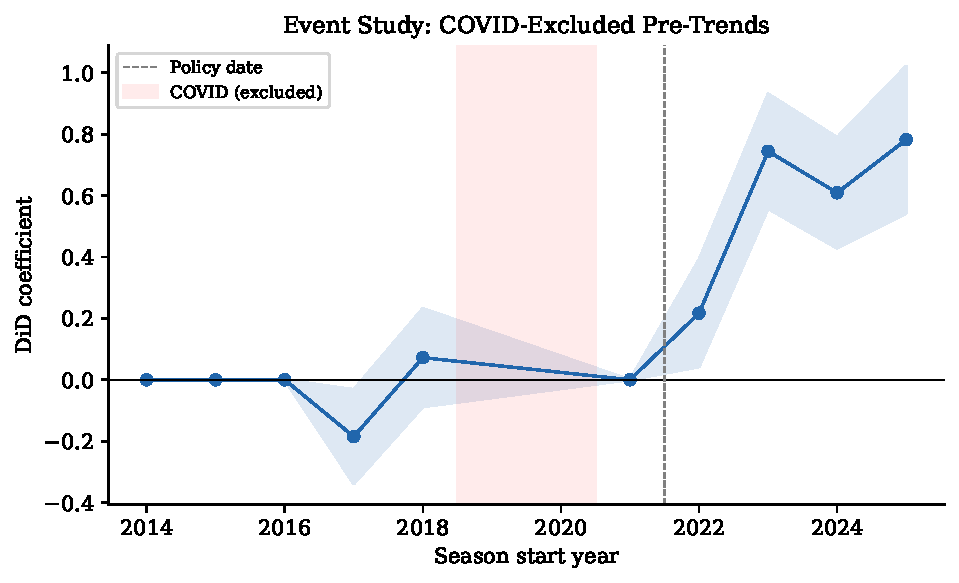
\includegraphics[width=0.85\textwidth]{fig_covid_pretrends_v3}
\caption{Event study excluding COVID-affected seasons (2019--20 and 2020--21). Pre-treatment coefficients remain significantly different from zero ($F = 6.94$, $p = 0.001$).}
\label{fig:covid_pretrends_v3}
\end{figure}


\subsection{The Premier League Reversal}
\label{subsec:pl_reversal}

The strongest causal evidence in our design is the English Premier League's partial reversal of the directive in 2024--25. Following widespread criticism from managers and players about excessive stoppages, the PGMOL (Professional Game Match Officials Limited) issued revised guidance for 2024--25, signaling a return toward shorter stoppage periods.\footnote{Multiple media reports from August 2024 confirm the PGMOL's revised approach. The explicit policy was framed not as a reversal of the FIFA directive but as a ``recalibration'' following feedback from clubs and match officials.} Figure~\ref{fig:pl_reversal} displays the trajectory of second-half stoppage time across the Big Five leagues.

\begin{figure}[H]
\centering
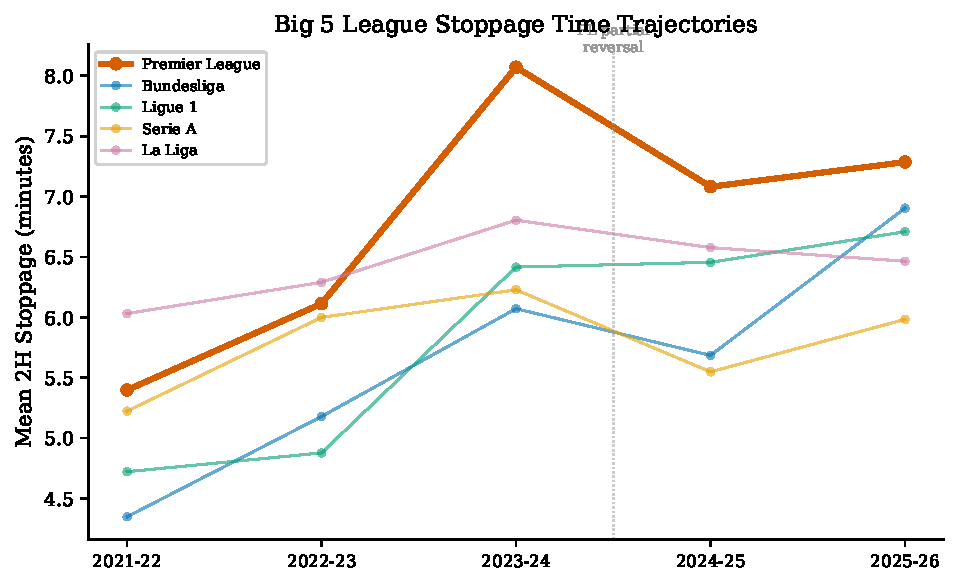
\includegraphics[width=\textwidth]{fig_pl_reversal}
\caption{Big Five league stoppage-time trajectories, 2021--22 through 2025--26. The Premier League (bold line) shows a sharp increase in 2023--24 followed by a partial reversal in 2024--25 ($-0.99$ minutes). Other leagues show more stable post-directive trajectories.}
\label{fig:pl_reversal}
\end{figure}

The Premier League's mean second-half stoppage fell from 8.07 minutes in 2023--24 to 7.08 minutes in 2024--25, a decline of 0.99 minutes. This decline is significantly larger than the changes in other Big Five leagues: the DiD estimate comparing the PL to the other four Big Five leagues is $\hat{\beta} = -0.660$ (SE $= 0.185$, $p < 0.001$). The within-country comparison to the Championship---which shares the PGMOL referee pool---yields $\hat{\beta} = -0.569$ (SE $= 0.199$, $p = 0.004$). The reversal represents approximately 37\% of the original increase from 2021--22 to 2023--24 ($+2.67$ minutes), suggesting a partial rather than complete pullback.

The reversal provides the closest analogue to a ``difference-in-differences-in-differences'' in our setting: a treated league that first increased and then partially reversed, while other treated leagues continued. This temporal pattern---increase following the directive, decrease following the recalibration---is difficult to reconcile with a secular-trend explanation and strengthens the case for a policy-driven effect.

Notably, goals scored after the 90th minute did not significantly decline in the PL relative to other Big Five leagues during the reversal ($\hat{\beta} = -0.042$, SE $= 0.038$, $p = 0.280$, $N = 3{,}486$). However, this null must be interpreted with appropriate caution: if the reversal was 37\% of the original stoppage increase, the expected late-goal reversal would be approximately 0.011 goals per match, and the test has only 6\% power to detect an effect of that magnitude (MDE at 80\% power $= 0.106$). The asymmetry---stoppage time reversed but late goals did not commensurately decline---is therefore \emph{underpowered} rather than definitive, and is consistent with either slow behavioral adaptation or simply an insufficiently large sample to detect a small reversal effect.


\subsection{Honest Assessment}
\label{subsec:honest_assessment}

The evidence supports a treatment effect in the range of 0.6--1.0 additional minutes, robust in sign across all specifications. However, the event study does not validate parallel trends (Section~\ref{subsec:pretrends_results}), and the \citet{rambachan2023more} breakdown value of $\bar{M}^* \approx 0$ means the result is not robust to meaningful extrapolation of pre-existing differential trends (Figure~\ref{fig:honest_did_v3}). This is the design's most consequential limitation.

Six considerations support proceeding with a causal interpretation. \textit{First}, the Premier League's partial reversal (Section~\ref{subsec:pl_reversal}) provides within-league temporal variation that is difficult to attribute to secular trends: the increase following the directive and the decrease following the recalibration track policy changes, not time trends. \textit{Second}, the within-country event study (Figure~\ref{fig:within_country_es}) shows the same pattern with country$\times$season fixed effects. \textit{Third}, the within-country strategy exploits the strongest institutional variation: shared referee pools, broadcasting infrastructure, and competitive calendars. \textit{Fourth}, permutation inference ($p = 0.045$) does not depend on parallel trends. \textit{Fifth}, the specification curve shows 88.8\% of 420 specifications produce significant positive estimates. \textit{Sixth}, leave-one-out analysis shows no single league drives the result.

As \citet{roth2022pretest} emphasize, when parallel trends cannot be validated, credibility rests on the institutional case. Readers who require $\bar{M}^* > 0$ should interpret our results as a precise descriptive accounting of what changed when enforcement norms shifted.


% ══════════════════════════════════════════════════════════════
%  WELFARE
% ══════════════════════════════════════════════════════════════
\section{Welfare Implications}
\label{sec:welfare}

The preceding sections have established the directive's effects on match
outcomes, scoring patterns, and market prices. We now turn to the
normative question: who gained, who lost, and on net, was the directive
welfare-improving? We examine four constituencies: consumers (fans and
viewers), workers (players), clubs (through competitive balance), and
broadcasters.

\subsection{Consumer Welfare: The Redistribution of Entertainment}
\label{subsec:consumer}

From the perspective of match-day entertainment, the directive's most
visible consequence was a dramatic increase in late-game drama. The pre-post
estimate for goals scored after the 90th minute corresponds to an
approximately 20 percent increase relative to the pre-directive mean, and
the probability of a game-changing goal in added time---a goal after
the 85th minute that alters the result---increased by a
similar magnitude in treated leagues. The probability that second-half stoppage exceeded eight
minutes rose from 7.1 percent to 27.8 percent in treated leagues, transforming the final
minutes from a brief coda into a substantive phase of play.

Yet total goals per match were unchanged. The entertainment ``budget,'' if
measured in goals, was redistributed rather than expanded: more late goals,
but commensurately fewer goals per minute during the expanded playing
time. Whether this redistribution increased consumer surplus depends on
the shape of the fan's utility function over goal timing. If fans value
dramatic, late-deciding goals disproportionately---a plausible assumption
given revealed preferences in media consumption---then the directive
improved the quality of the viewing experience while holding quantity
fixed. We note, however, that this assessment is qualitative; we have no
direct measure of willingness to pay or viewership response.

A back-of-envelope calculation quantifies the scale. With an average attendance of approximately 26{,}000 per match across treated leagues in the post-directive period and roughly 1{,}530 matches per season, the directive generates approximately \textbf{1.0 million additional fan-hours} of clock time per season ($1.56 \text{ min} \times 1{,}530 \text{ matches} \times 26{,}000 \text{ fans} / 60 \approx 1{,}034{,}000$ hours).\footnote{This represents clock time, not ball-in-play time. Effective playing time is typically 55--60\% of clock time, so the additional active play is approximately 570,000--620,000 fan-hours.} An additional ${\sim}46$ goals are scored after the 90th minute per season (DiD estimate of $+0.030$ per match $\times$ 1,530 matches), and the proportion of matches featuring at least one late goal rose from 14.7\% to 19.2\% ($+4.5$ percentage points). These are meaningful effects at scale.

From a broadcasting perspective, the directive increased the duration of
live match coverage by approximately 1.6 minutes per match in the most-treated
leagues. This expansion creates additional advertising inventory and, more
importantly, extends the window during which audiences remain engaged.\footnote{A back-of-envelope revenue estimate: the $1.6 \times 1{,}530 \approx 2{,}450$ additional broadcast minutes across Big Five leagues, benchmarked against aggregate domestic rights of approximately EUR~6.5B per season, yield EUR~107M at linear per-minute valuation and EUR~54M with a 50\% marginal-minute discount.}

\subsection{Worker Welfare: Player Health and Workload}
\label{subsec:worker}

The directive's most direct labor-market consequence was an increase in
per-match workload. Our player-level estimates indicate an increase of
$0.76$ minutes per match per player (SE~$= 0.145$, $p < 0.001$,
$N = 830{,}569$ player-match observations; standard errors clustered at
the league level). Over a season, this
accumulates to a non-trivial increase in total playing time, raising
legitimate concerns about fatigue and injury risk---concerns echoed in the
sports medicine literature \citep{mohr2023extended} and the broader
evidence on overtime and occupational injuries \citep{dembe2005effect},
and voiced prominently by players' unions \citep{fifpro2023workload}.

The injury evidence, however, tells a more nuanced story. Total injuries
per player-season \emph{decreased} following the directive ($\beta =
-0.090$, SE~$= 0.032$, $p = 0.005$; pre-treatment mean $= 1.886$). This
counterintuitive finding admits several explanations. First, if the
stable total-goals result (Section~\ref{subsec:decomposition}) reflects
genuine behavioral pacing, the reduced intensity may have lowered
biomechanical stress per unit of playing time.
Second, the longer stoppage periods may have provided de facto recovery
windows. Third, the finding may
reflect confounding changes in squad rotation or fixture scheduling that
coincided with the directive.

The most policy-relevant test concerns muscular injuries specifically,
since these are the injury type most directly linked to workload and
fatigue. The DiD estimate for muscular injuries is
$\beta = -0.007$ (SE~$= 0.019$, $p = 0.73$; pre-treatment mean $=
0.525$).\footnote{Injury regressions use HC1 robust standard errors at the player-season level rather than the league-clustered SEs used in the main specification, because the injury panel covers only 9 leagues. With 9 clusters, league-clustered inference would produce wider confidence intervals, further strengthening the null.} This null is well-powered: our design has 88.6 percent power to
detect a 10 percent increase in muscular injury rates, based on
$N = 23{,}255$ player-seasons. The data are therefore informative enough
to reject a clinically meaningful increase, and we conclude that there is
no evidence that the directive harmed player welfare through increased
muscular injury risk.

We emphasize appropriate caution in interpreting these results. The injury
decrease could reflect time-varying confounders---improvements in sports
medicine, changes in training protocols, or strategic rest
patterns---that coincided with but were not caused by the directive.
Our identification strategy absorbs league and season fixed effects but
cannot rule out within-league temporal shocks correlated with the
directive's adoption. The most defensible claim is that the directive did
not \emph{measurably worsen} the injury environment, not that it improved
it (Figure~\ref{fig:injury_rates_v3} in Appendix~\ref{app:figures}).

\subsection{Aggregate Assessment}

The evidence is consistent with a modestly positive welfare effect.
Consumers received approximately 1.0 million additional fan-hours per season and
a 4.5 percentage-point increase in the share of matches featuring at least one goal after the 90th minute, at no
cost in total match quality. Players worked slightly more per match ($+0.76$ min)
but did not experience higher injury rates. Competitive balance was unaffected.
The foul rate per minute declined within treated leagues, though the DiD estimate is positive ($+1.24$ fouls, $p < 0.001$), indicating that treated leagues experienced a \emph{smaller} secular foul decline than controls. We attribute the foul-rate decline to period effects common to all leagues rather than the directive itself (Section~\ref{subsec:decomposition}).
We find no evidence that any measured constituency was made worse off, though
our tests have limited power for some welfare-relevant outcomes
(particularly viewership and broadcaster revenues, which we do not
observe).


% ══════════════════════════════════════════════════════════════
%  CONCLUSION
% ══════════════════════════════════════════════════════════════
\section{Conclusion}
\label{sec:conclusion}

This paper has studied a natural experiment in time regulation: FIFA's
2022 directive instructing referees to add substantially more stoppage
time to professional football matches. The directive expanded effective
playing time by 0.7--1.6 minutes per match depending on the specification,
a large and sudden change to the temporal structure of a globally
significant economic activity. Our central finding is that this expansion
of the competitive window did not increase total goal production. Instead,
it redistributed goals from regulation time into added time: the overall per-minute
scoring rate was unchanged at 0.028 goals/minute ($p = 0.47$), with rates in added time
similarly stable ($p = 0.68$), and total goals per match were unchanged despite the additional minutes.

The quantity-intensity pattern constitutes the paper's core contribution.
The directive created more competitive time, yet total goals were unchanged.
Whether this reflects active behavioral adaptation (effort reallocation) or
compositional effects (added time being inherently lower-productivity) remains
an open question. Either way, the result echoes the labor-economics findings of
\citet{pencavel2015effects} on the concavity of the hours-output
relationship: extending the work period did not proportionally increase
output, regardless of the mechanism.

The finding also connects loosely to end-game effects in market design \citep{rothockenfels2002}, though the mechanism differs: whereas auction sniping reflects strategic response to a hard deadline, the displacement we document is primarily mechanical (more minutes at a similar rate) rather than strategic repositioning.

The policy implications extend beyond football. The directive achieved its
stated goal---more effective playing time---without disrupting the sport's
low-scoring character, competitive balance, or player health. The implicit offset---total output unchanged despite more time---implies that
regulators may have more latitude to modify temporal rules than naive
extrapolation would suggest, precisely because total output is less
elastic to duration than a linear model would predict.

We close with the design's fundamental limitation, which readers should weigh when assessing our causal claims. The event study rejects parallel pre-trends ($F = 9.0$, $p < 0.001$), and the \citet{rambachan2023more} breakdown value is $\bar{M}^* \approx 0$: the treatment effect is not robust to meaningful extrapolation of pre-treatment trends. Moreover, because the directive's transmission ran through shared refereeing bodies, no league in our sample was fully untreated---control leagues increased stoppage by 0.89 minutes on average. This creates a SUTVA concern: within-country pairs like the Premier League and the Championship share a referee pool (PGMOL), meaning the ``control'' division received a diluted version of the same treatment rather than no treatment at all. Our estimates should therefore be interpreted as lower bounds of the true treatment effect, and the identification relies on \emph{differential} enforcement intensity rather than a clean treated-control contrast. The permutation inference ($p = 0.045$), specification curve (88.8\% of 420 specifications significant), and institutional evidence provide supporting identification, but the pre-trend failure means that readers who require classical parallel-trends validation will not find it here.

The English Premier League's partial reversal of the directive in 2024--25 provides a natural test of symmetry (Section~\ref{subsec:pl_reversal}). The PL's stoppage time declined by 0.99 minutes, a highly significant reversal relative to both the other Big Five leagues ($p < 0.001$) and the Championship ($p = 0.004$). Yet goals scored after the 90th minute did not commensurately decline ($p = 0.280$), though this test is substantially underpowered (6\% power at the expected effect size). Whether the asymmetry reflects slow behavioral adaptation, structural changes in late-game play patterns, or simply insufficient sample size is a question for future work.


% ══════════════════════════════════════════════════════════════
%  REFERENCES
% ══════════════════════════════════════════════════════════════
\singlespacing
\bibliography{references}


% ══════════════════════════════════════════════════════════════
%  APPENDIX
% ══════════════════════════════════════════════════════════════
\clearpage
\begin{appendices}

\section{Referee Compliance Details}
\label{app:compliance}

Table~\ref{tab:compliance_v3} reports detailed compliance statistics at the referee, match, and convergence levels.

\begin{table}[htbp]
\centering
\caption{Referee Compliance Analysis}
\label{tab:compliance_v3}
\begin{threeparttable}
\begin{tabular}{lrrr}
\toprule
& \multicolumn{1}{c}{$N$} & \multicolumn{1}{c}{Rate} & \multicolumn{1}{c}{$\Delta$ (min)} \\
\midrule
\multicolumn{4}{l}{\textit{Panel A: Referee-Level Compliance}} \\
  $\geq 20$ matches pre \& post & 85 & 100.0\% & +1.46 \\
  $\geq 10$ matches pre \& post & 102 & 98.0\% & +1.40 \\
  Any pre \& post matches & 120 & 95.0\% & +1.31 \\
\midrule
\multicolumn{4}{l}{\textit{Panel B: Match-Level Compliance (Post-Policy Treated)}} \\
  Above league pre-median & 4596 & 70.2\% & --- \\
  Above league pre-mean & 4596 & 73.3\% & --- \\
\midrule
\multicolumn{4}{l}{\textit{Panel C: Convergence (CV of Ref.\ Stoppage)}} \\
  Pre-policy CV & --- & 0.173 & --- \\
  Post-policy CV & --- & 0.144 & --- \\
\bottomrule
\end{tabular}
\begin{tablenotes}[flushleft]\footnotesize
\item \textit{Notes:} Referee-level compliance = share of referees whose post-policy mean 2H stoppage exceeds their pre-policy mean. Match-level compliance = share of post-policy treated matches exceeding the league's pre-policy median 2H stoppage. CV = coefficient of variation across referee means.
\end{tablenotes}
\end{threeparttable}
\end{table}

\section{Player Health and Workload}
\label{app:health}

Table~\ref{tab:health_v3} reports DiD estimates for injury outcomes (Panel~A), injury rates per 1,000 minutes (Panel~B), match-level workload (Panel~C), and season-level workload (Panel~D).

\begin{table}[htbp]
\centering
\begin{threeparttable}
\caption{Player Health and Workload Effects of the Stoppage-Time Directive}
\label{tab:health_v3}
\begin{tabular}{lccccc}
\toprule
& $\hat{\beta}_{\text{DiD}}$ & SE & Pre mean & $N$ & $R^2$ \\
\midrule
\addlinespace
\multicolumn{6}{l}{\textit{Panel A: Injury outcomes (player-season)}} \\
\addlinespace[3pt]
\quad Total injuries & $-0.0900^{**}$ & (0.0318) & 1.886 & 23,255 & 0.0451 \\
\quad Muscular injuries & $-0.0067$ & (0.0194) & 0.525 & 23,255 & 0.0377 \\
\quad Days absent & $+0.8944$ & (2.6029) & 66.522 & 23,255 & 0.0239 \\
\quad Games missed & $+0.3288$ & (0.3138) & 8.695 & 23,255 & 0.0334 \\
\quad High severity ($>$28d) & $-0.0185$ & (0.0141) & 0.506 & 23,255 & 0.0360 \\
\quad Has recurrence & $-0.0173$ & (0.0126) & 0.286 & 23,255 & 0.0383 \\
\addlinespace
\multicolumn{6}{l}{\textit{Panel B: Injury rates (per 1,000 minutes)}} \\
\addlinespace[3pt]
\quad All injuries / 1000 min & $+0.1460$ & (1.5571) & 5.770 & 21,088 & 0.0062 \\
\quad Muscular / 1000 min & $+0.2385$ & (0.3619) & 1.270 & 21,088 & 0.0009 \\
\addlinespace
\multicolumn{6}{l}{\textit{Panel C: Workload (player-match level)}} \\
\addlinespace[3pt]
\quad Minutes per match & $+0.7644^{***}$ & (0.1449) & --- & 830,569 & 0.0139 \\
\quad Stoppage exposure (min) & $+0.6078^{***}$ & (0.0215) & --- & 830,569 & 0.2133 \\
\quad Days since last match & $+0.2320^{**}$ & (0.0883) & --- & 816,557 & 0.0084 \\
\addlinespace
\multicolumn{6}{l}{\textit{Panel D: Workload (player-season level)}} \\
\addlinespace[3pt]
\quad Total minutes / season & $-70.5^{**}$ & (27.1) & --- & 21,088 & 0.0387 \\
\quad Total matches / season & $-1.0092^{***}$ & (0.2916) & --- & 21,088 & 0.0529 \\
\quad Avg days between matches & $-0.0487$ & (0.4363) & --- & 20,758 & 0.0171 \\
\bottomrule
\end{tabular}
\begin{tablenotes}[flushleft]
\footnotesize
\item \textit{Notes:} DiD estimates with league and season fixed effects.
Panel~A reports injury outcomes at the player-season level.
Panel~B conditions on players with non-zero minutes and reports
injury rates per 1,000 playing minutes.
Panels~C and~D report workload at the player-match and player-season
levels, respectively. ``Pre mean'' is the treated-group pre-policy average.
Robust standard errors (HC1) in parentheses.
$^{*}p<0.05$, $^{**}p<0.01$, $^{***}p<0.001$.
\end{tablenotes}
\end{threeparttable}
\end{table}

\section{Additional Figures}
\label{app:figures}

\begin{figure}[H]
\centering
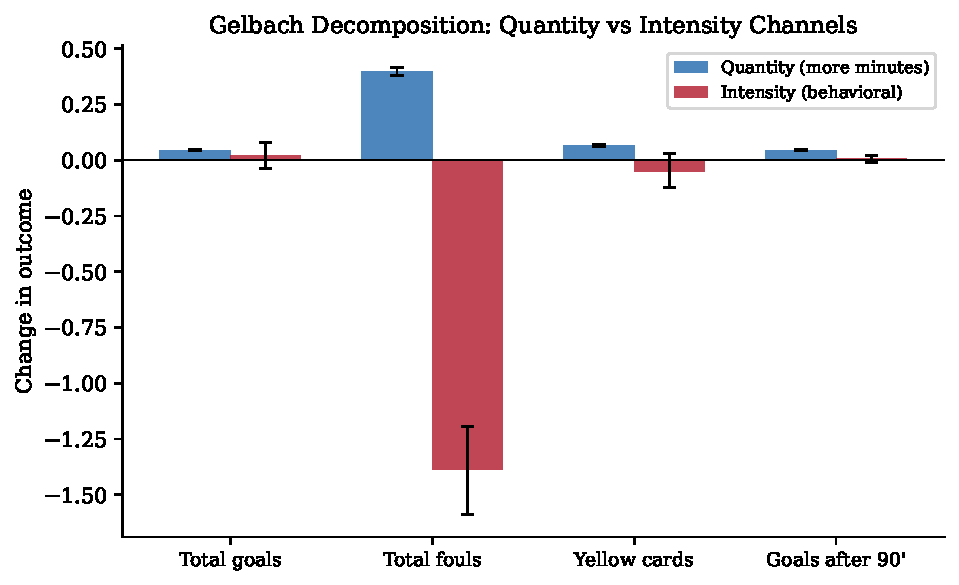
\includegraphics[width=0.85\textwidth]{fig_decomposition_v3}
\caption{Quantity--intensity decomposition for each outcome. Blue bars show the expected change from additional minutes at the pre-treatment rate; red bars show the behavioral intensity residual. Error bars are bootstrap 95\% CIs.}
\label{fig:decomposition_v3}
\end{figure}

\begin{figure}[H]
\centering
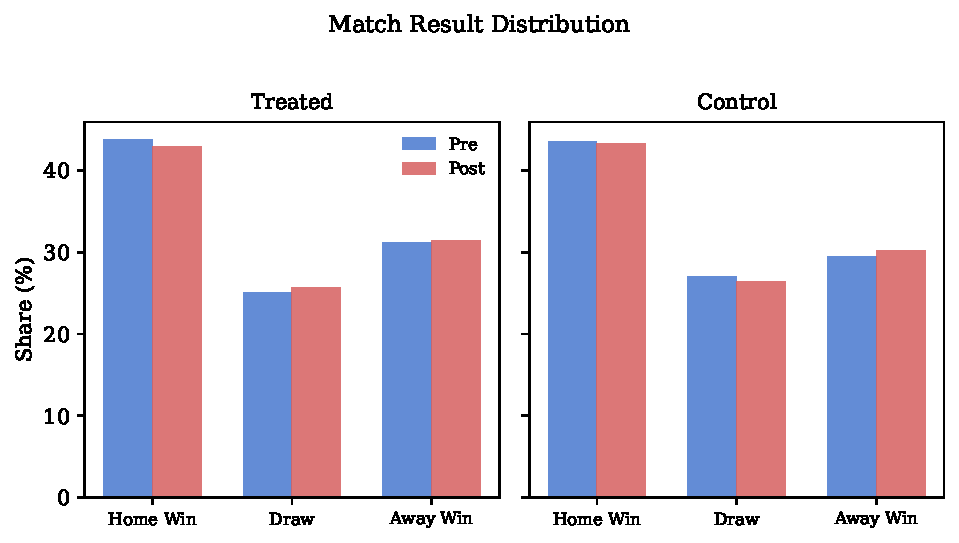
\includegraphics[width=0.85\textwidth]{fig_result_changes_v3}
\caption{Distribution of match result changes in stoppage time, pre- vs.\ post-directive.}
\label{fig:result_changes_v3}
\end{figure}

\begin{figure}[H]
\centering
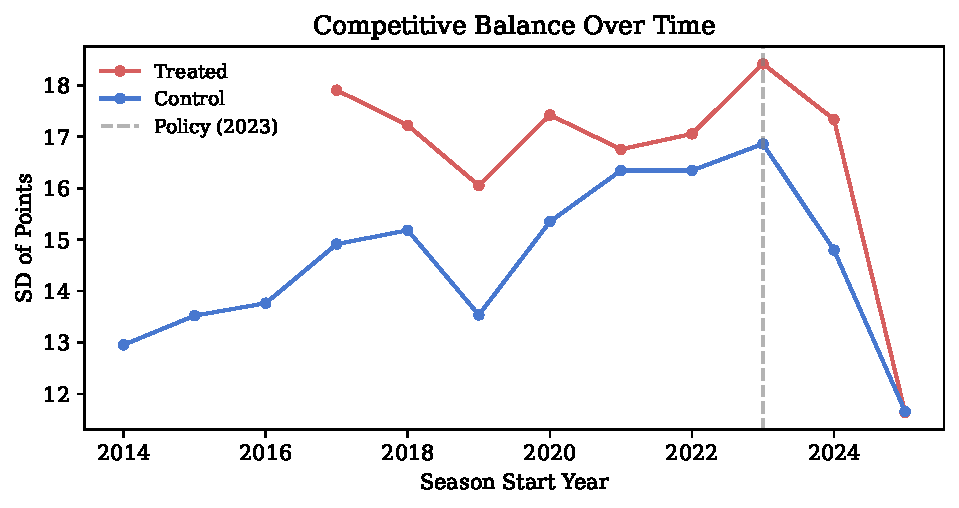
\includegraphics[width=0.85\textwidth]{fig_competitive_balance_v3}
\caption{Competitive balance measures (standard deviation of points and normalized HHI) by season, treated vs.\ control leagues.}
\label{fig:competitive_balance_v3}
\end{figure}

\begin{figure}[H]
\centering
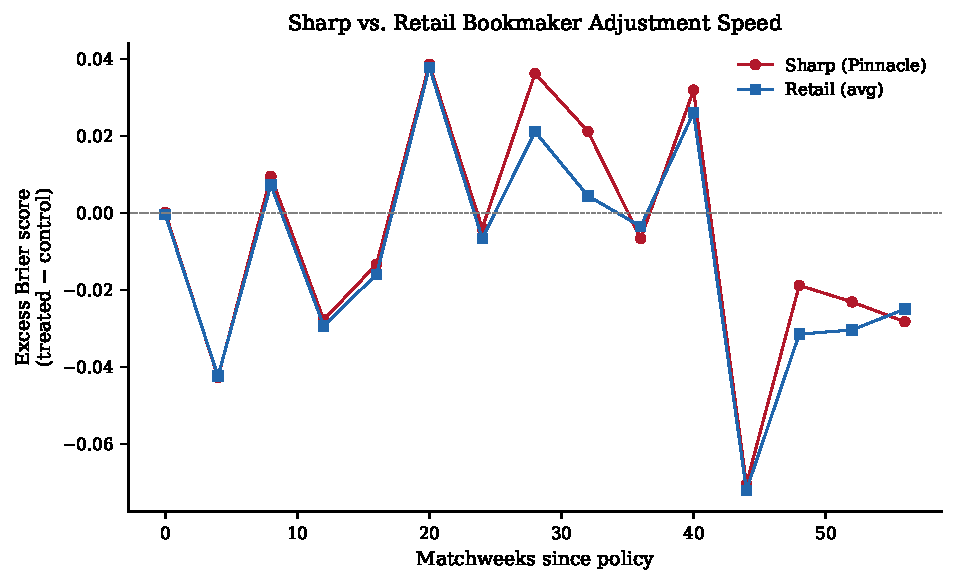
\includegraphics[width=0.85\textwidth]{fig_bookmaker_adjustment_v3}
\caption{Betting market adjustment speed: week-by-week Brier score excess post-directive, by bookmaker.}
\label{fig:bookmaker_adjustment_v3}
\end{figure}

\begin{figure}[H]
\centering
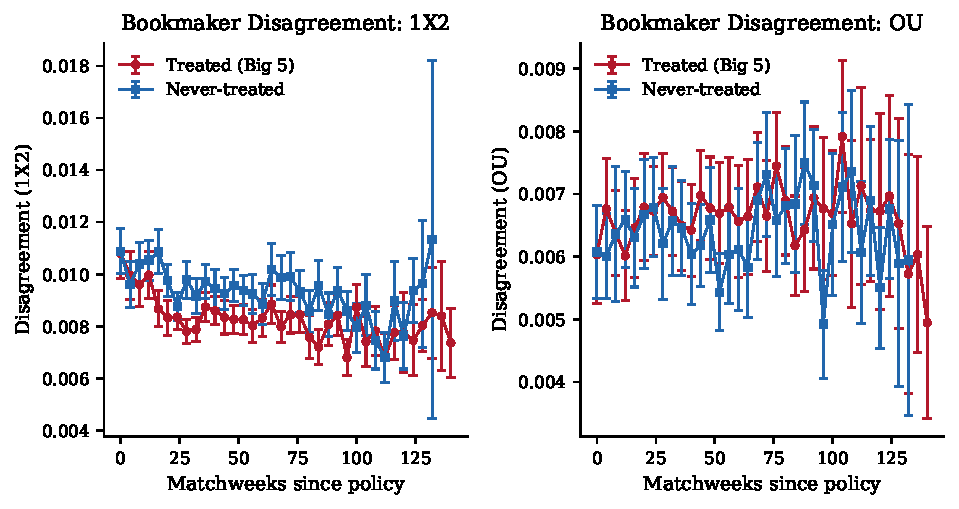
\includegraphics[width=0.85\textwidth]{fig_odds_spread_v3}
\caption{Sharp--retail odds spread (Pinnacle vs.\ Bet365) over time.}
\label{fig:odds_spread_v3}
\end{figure}

\begin{figure}[H]
\centering
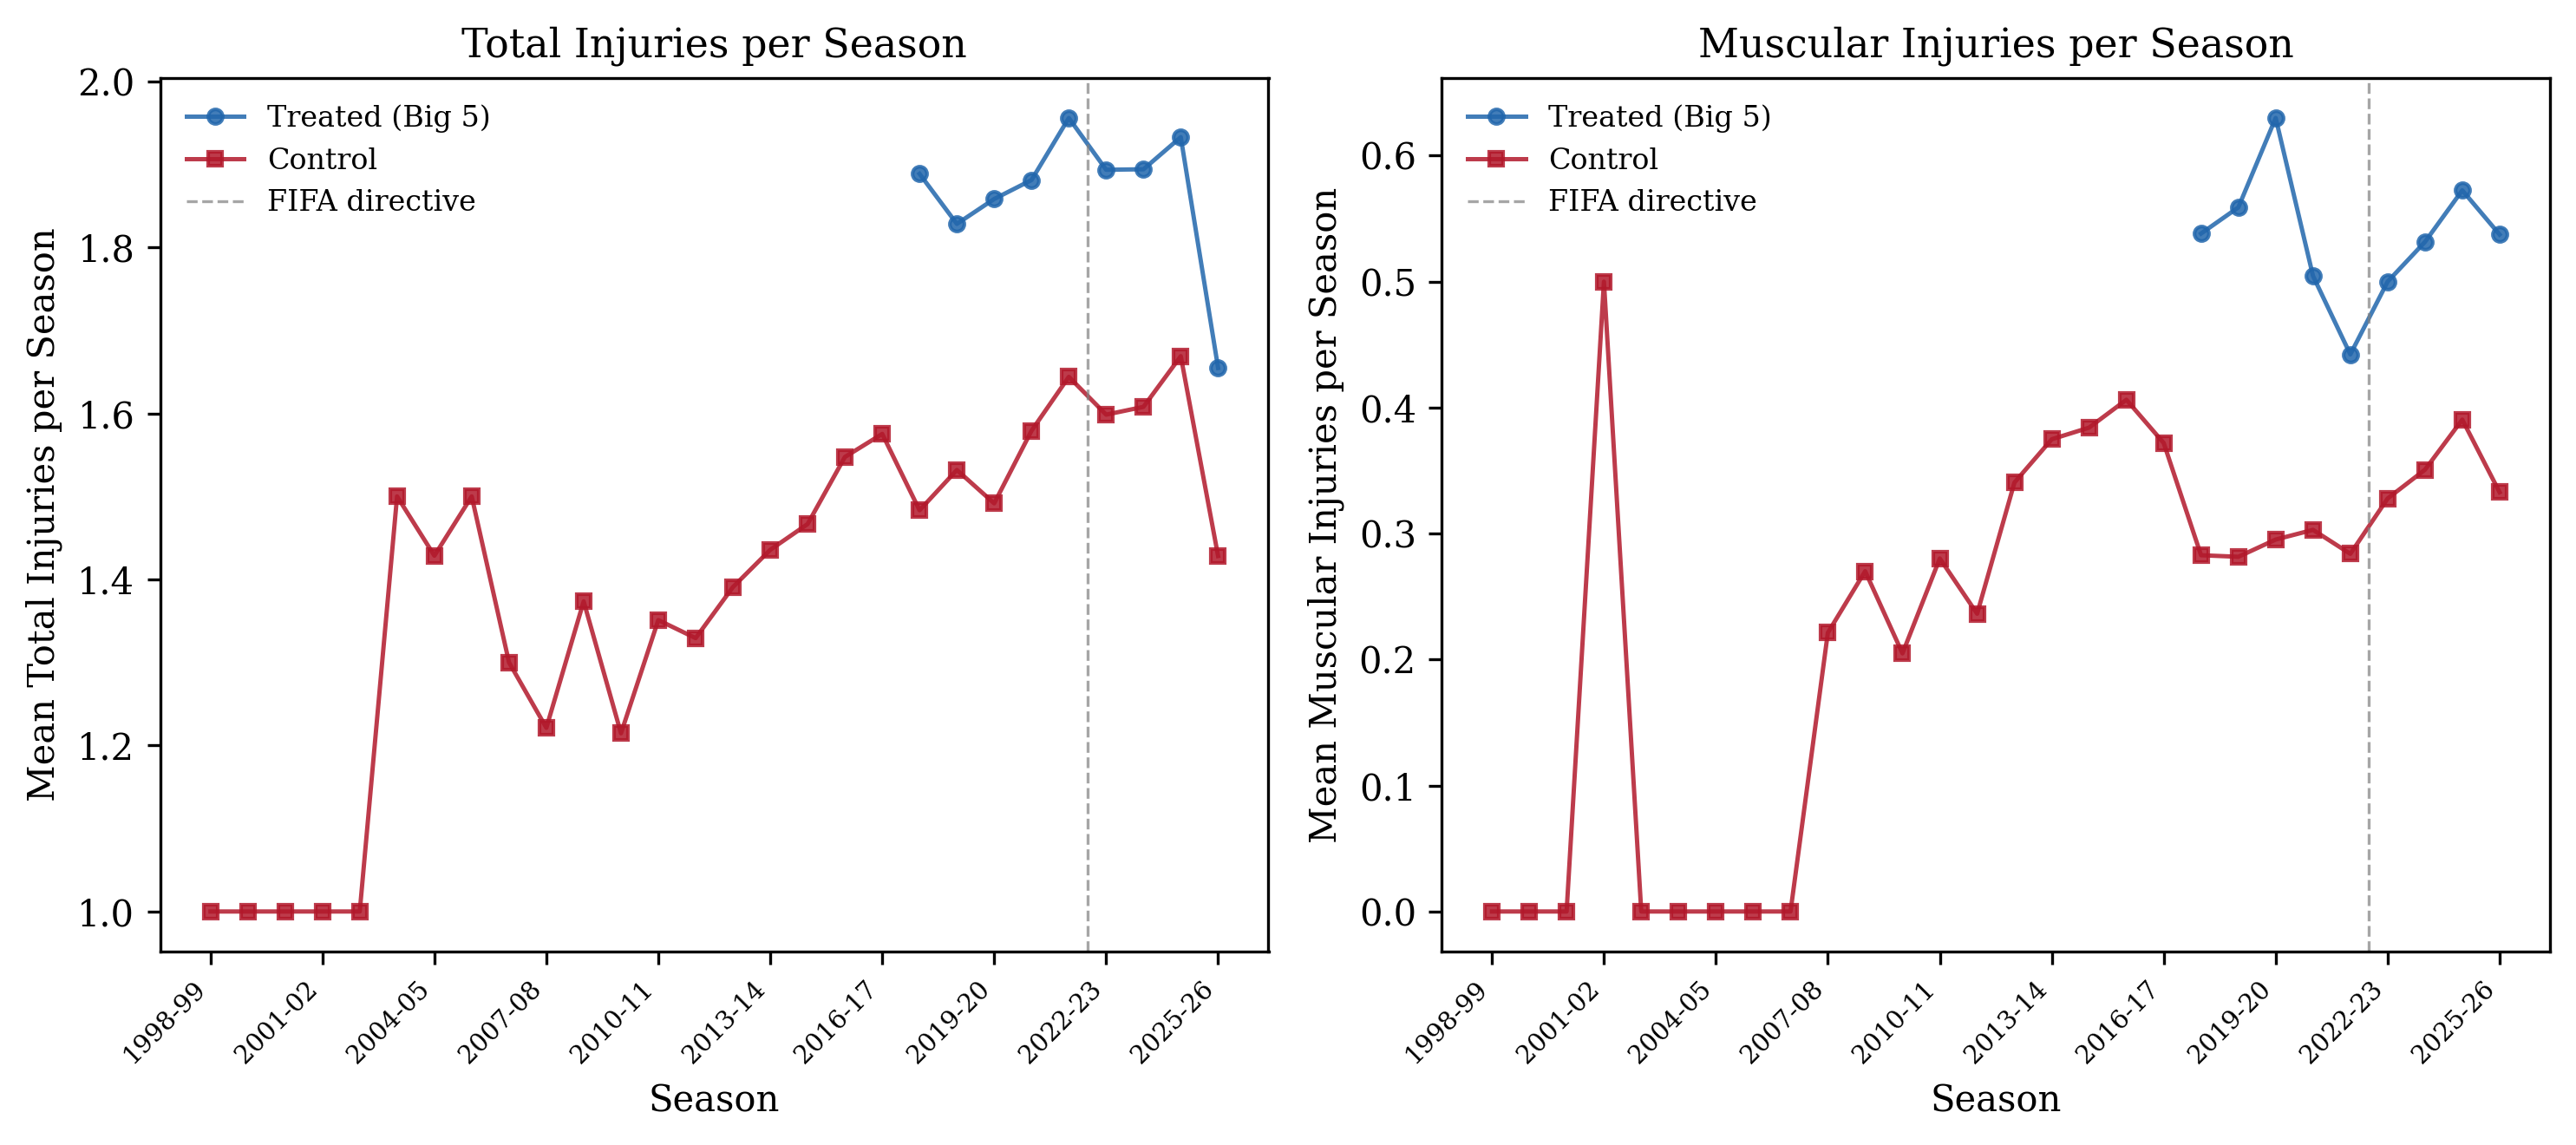
\includegraphics[width=0.85\textwidth]{fig_injury_rates_v3}
\caption{Injury rates per 1,000 player-minutes, pre- vs.\ post-directive, by injury type.}
\label{fig:injury_rates_v3}
\end{figure}

\end{appendices}

\end{document}
